% --------------------------------------------------------
% DEFINIÇÕES DO DOCUMENTO
% --------------------------------------------------------

\documentclass[
	% -- opções da classe memoir --
	12pt,				% tamanho da fonte
	openright,			% capítulos começam em pág ímpar (insere página vazia caso preciso)
	oneside,			% para impressão em verso e anverso. Oposto a oneside
	a4paper,			% tamanho do papel. 
	% -- opções da classe abntex2 --
	%chapter=TITLE,		% títulos de capítulos convertidos em letras maiúsculas
	%section=TITLE,		% títulos de seções convertidos em letras maiúsculas
	%subsection=TITLE,	% títulos de subseções convertidos em letras maiúsculas
	%subsubsection=TITLE,% títulos de subsubseções convertidos em letras maiúsculas
	% -- opções do pacote babel --
	english,			% idioma adicional para hifenização
	french,				% idioma adicional para hifenização
	spanish,			% idioma adicional para hifenização
	brazil,				% o último idioma é o principal do documento
	]{abntex2}

% --------------------------------------------------------
% PACOTES
% --------------------------------------------------------

\usepackage{cmap}				% Mapear caracteres especiais no PDF
\usepackage{lmodern}			% Usa a fonte Latin Modern			
\usepackage[T1]{fontenc}		% Selecao de codigos de fonte.
\usepackage[utf8]{inputenc}		% Codificacao do documento (conversão automática dos acentos)
\usepackage{lastpage}			% Usado pela Ficha catalográfica
\usepackage{indentfirst}		% Indenta o primeiro parágrafo de cada seção.
\usepackage{color}				% Controle das cores
\usepackage{graphicx}			% Inclusão de gráficos
\usepackage{lipsum}				% para geração de dummy text
\usepackage[brazilian,hyperpageref]{}	 % Paginas com as citações na bibl
\usepackage[alf]{abntex2cite}	% Citações padrão ABNT
\usepackage[br]{nicealgo}       % Pacote para criação de algoritmos
\usepackage{customizacoes}      % Pacote de customizações do abntex2


% --------------------------------------------------------
% CONFIGURAÇÕES DE PACOTES
% --------------------------------------------------------

% Configurações do pacote backref
\renewcommand{\familydefault}{\sfdefault}
% Usado sem a opção hyperpageref de backref
% \renewcommand{\backrefpagesname}{Citado na(s) página(s):~}
% Texto padrão antes do número das páginas
% \renewcommand{\backref}{}
% Define os textos da citação
% \renewcommand*{\backrefalt}[4]{
	% \ifcase #1 %
		% Nenhuma citação no texto.%
	% \or
		% Citado na página #2.%
	% \else
		% Citado #1 vezes nas páginas #2.%
	% \fi}%


% --------------------------------------------------------
% INFORMAÇÕES DE DADOS PARA CAPA E FOLHA DE ROSTO
% --------------------------------------------------------

\titulo{Utilização de técnicas de Machine Learning para Detecção de Botnets}
\autor{Luis Felipe Bueno da Silva}
\local{Bauru}
\data{2018}
\orientador{Prof. Dr. Kelton Augusto Pontara da Costa}
\instituicao{%
  Universidade Estadual Paulista ``Júlio de Mesquita Filho''
  \par
  Faculdade de Ciências
  \par
  Ciência da Computação}
\tipotrabalho{Trabalho de Conclusão de Curso}
\preambulo{Trabalho de Conclusão de Curso do Curso de Ciência da Computação da Universidade Estadual Paulista ``Júlio de Mesquita Filho'', Faculdade de Ciências, Campus Bauru.}


% --------------------------------------------------------
% CONFIGURAÇÕES PARA O PDF FINAL
% --------------------------------------------------------

% alterando o aspecto da cor azul
\definecolor{blue}{RGB}{41,5,195}

% informações do PDF
\makeatletter
\hypersetup{
     	%pagebackref=true,
		pdftitle={\@title}, 
		pdfauthor={\@author},
    	pdfsubject={\imprimirpreambulo},
	    pdfcreator={LaTeX with abnTeX2},
		pdfkeywords={abnt}{latex}{abntex}{abntex2}{trabalho acadêmico}, 
		colorlinks=true,       		% false: boxed links; true: colored links
    	linkcolor=blue,          	% color of internal links
    	citecolor=blue,        		% color of links to bibliography
    	filecolor=magenta,      		% color of file links
		urlcolor=blue,
		bookmarksdepth=4
}
\makeatother


% --------------------------------------------------------
% ESPAÇAMENTOS ENTRE LINHAS E PARÁGRAFOS
% --------------------------------------------------------

% O tamanho do parágrafo é dado por:
\setlength{\parindent}{1.3cm}

% Controle do espaçamento entre um parágrafo e outro:
\setlength{\parskip}{0.2cm}


% --------------------------------------------------------
% COMPILANDO O ÍNDICE
% --------------------------------------------------------

\makeindex


% --------------------------------------------------------
% INÍCIO DO DOCUMENTO
% --------------------------------------------------------

\begin{document}

% Seleciona o idioma do documento (conforme pacotes do babel)
\selectlanguage{brazil}

% Retira espaço extra obsoleto entre as frases.
\frenchspacing 


% --------------------------------------------------------
% ELEMENTOS PRÉ-TEXTUAIS
% --------------------------------------------------------

% Capa
\imprimircapa

% Folha de rosto
% (o * indica que haverá a ficha bibliográfica)
\imprimirfolhaderosto*

% Inserir a ficha bibliografica
\begin{fichacatalografica}
	\sffamily
	\vspace*{\fill}					% Posição vertical
	\begin{center}					% Minipage Centralizado
	\fbox{\begin{minipage}[c][8cm]{15.5cm}		% Largura
	\small
	\imprimirautor
	\hspace{0.5cm} \imprimirtitulo  / \imprimirautor. --
	\imprimirlocal, \imprimirdata-
	\hspace{0.5cm} \pageref{LastPage} p. : il. (algumas color.) ; 30 cm.\\
	\hspace{0.5cm} \imprimirorientadorRotulo~\imprimirorientador\\
	\hspace{0.5cm}
	\parbox[t]{\textwidth}{\imprimirtipotrabalho~--~\imprimirinstituicao,
	\imprimirdata.}\\
	\hspace{0.5cm}
		1. Botnet
		2. Machine Learning
		3. Inteligência Artificial
		4. Python
	\end{minipage}}
	\end{center}
\end{fichacatalografica}

% Inserir folha de aprovação
\begin{folhadeaprovacao}
  \begin{center}
    {\ABNTEXchapterfont\large\imprimirautor}
    \vspace*{\fill}\vspace*{\fill}
    \begin{center}
      \ABNTEXchapterfont\bfseries\Large\imprimirtitulo
    \end{center}
    \vspace*{\fill}
    \hspace{.45\textwidth}
    \begin{minipage}{.5\textwidth}
        \imprimirpreambulo
    \end{minipage}%
    \vspace*{\fill}
   \end{center}
   \center Banca Examinadora
   \assinatura{\textbf{\imprimirorientador} \\ Orientador} 
   \assinatura{\textbf{Profª. Drª. Simone das Graças Domingues Prado} \\ Convidado 1}
   \assinatura{\textbf{Professor} \\ Convidado 2}
   \begin{center}
    \vspace*{0.5cm}
    \par
    {Bauru, \_\_\_\_\_ de \_\_\_\_\_\_\_\_\_\_\_ de \_\_\_\_.}
    \vspace*{1cm}
  \end{center}
\end{folhadeaprovacao}

% % Dedicatória
% \begin{dedicatoria}
%   \vspace*{\fill}
%   \centering
%   \noindent
%   \textit{Espaço destinado à dedicátoria do texto.} \vspace*{\fill}
% \end{dedicatoria}

% Agradecimentos
\begin{agradecimentos}

Espaço reservado para agradecimentos.

\end{agradecimentos}

% Epígrafe
\begin{epigrafe}
    \vspace*{\fill}
	\begin{flushright}
		"The ending isn’t any more important \linebreak \rightline{than any of the moments leading to it}" \newline 
		(To the Moon) 
	\end{flushright}
\end{epigrafe}


% --------------------------------------------------------
% RESUMOS
% --------------------------------------------------------

% resumo em português
\setlength{\absparsep}{18pt} % ajusta o espaçamento dos parágrafos do resumo
\begin{resumo}
Esta monografia busca apresentar o estudo de métodos da área de \textit{Machine Learning} aplicados para a área de detecção de Botnets, redes de computadores comprometidos que são controlados por um invasor com o fim de executar atividades como ataques \textit{DDoS}, roubos de dados, entre outras ações maliciosas. Este trabalho é focado em estudar a eficiências dos classificadores mais utilizados em estudos anteriores da área, utilizando as técnicas de \textit{Naive Bayes}, \textit{Support Vector Machines}, Árvores de Decisão, Florestas Aleatórias, \textit{AdaBoost}, e aplicar técnicas para seleção de características de rede mais relevantes na tarefa de seleção dos tráfegos de Botnet em um ambiente de rede, através de uma abordagem de força bruta e uma abordagem utilizando o algoritmo de seleção de características \textit{Recursive Feature Elimination}. Busca também estudar a relevância de técnicas de otimização de hiper-parâmetros dos estimadores, com o objetivo de aumentar a acurácia. Por fim, são tiradas conclusões com base nos resultados obtidos no estudo. \linebreak
\textbf{Palavras-chave:} Botnet, Machine Learning, Inteligência Artificial, Python.
\end{resumo}

% resumo em inglês
\begin{resumo}[Abstract]
 \begin{otherlanguage*}{english}
This monograph presents the study of Machine Learning methods applied to the detection of Botnets, compromised computer networks that are controlled by an attacker in order to perform malicious activities such as DDoS attacks, data theft, among others. This work is focused on studying the efficiency of the most used classifiers in previous studies of the aream with the application of Naive Bayes, Support Vector Machines, Decision Trees, Random Forests and AdaBoost models, and apply techniques to select the most relevant network characteristics in the task of selecting botnet traffic in a network environment, through a brute-force approach and using the Recursive Feature Elimination algorithm. It also seeks to study the relevance of optimization techniques on estimators hyper-parameters, in order to increase model accuracy. Finally, conclusions are drawn based on the results obtained in the study. \linebreak
\textbf{Keywords:} Botnet, Machine Learning, Artificial Intelligence, Python.
 \end{otherlanguage*}
\end{resumo}


% --------------------------------------------------------
% LISTA DE ILUSTRAÇÕES
% --------------------------------------------------------

% inserir lista de ilustrações
\pdfbookmark[0]{\listfigurename}{lof}
\listoffigures*
\cleardoublepage


% --------------------------------------------------------
% LISTA DE TABELAS
% --------------------------------------------------------

% inserir lista de tabelas
\pdfbookmark[0]{\listtablename}{lot}
\listoftables*
\cleardoublepage


% --------------------------------------------------------
% LISTA DE ABREVIATURAS E SIGLAS
% --------------------------------------------------------

% inserir lista de abreviaturas e siglas
\begin{siglas}
  \item [CSV] \textit{Comma-separated Values} 
  \item [PCAP] \textit{Packet Capture}
  \item[SVM] \textit{Support Vector Machines}
  \item[RFE] \textit{Recursive Feature Elimination}
  \item[IA] Inteligência Artificial
  \item[ML] \textit{Machine Learning}
  \item[CV] \textit{Cross Validation}
  \item[NB] \textit{Naive Bayes}
  \item[UDP] \textit{User Datagram Protocol}
  \item[TCP] \textit{Transmission Control Protocol}
  \item[IAT] \textit{Inter-Arrival Time}
  \item[P2P] \textit {Peer to Peer}
  \item[C\&C] Comando e Controle
  \item[HTTP] \textit{Hypertext Transfer Protocol}
  \item[HTTPS] \textit{Hypertext Transfer Protocol Secure}
  \item[IRC] \textit{Internet Relay Chat}
\end{siglas}

% --------------------------------------------------------
% LISTA DE SÍMBOLOS
% --------------------------------------------------------

% inserir lista de símbolos
\begin{simbolos}
  \item[$ \gamma $] Letra grega Gama
\end{simbolos}


% --------------------------------------------------------
% SUMÁRIO
% --------------------------------------------------------

% inserir o sumario
\pdfbookmark[0]{\contentsname}{toc}
\tableofcontents*
\cleardoublepage


% --------------------------------------------------------
% ELEMENTOS TEXTUAIS
% --------------------------------------------------------

\pagestyle{simple}

% Arquivos .tex do texto, podendo ser escritos em um único arquivo ou divididos da forma desejada
\chapter{Introdução}
\label{c.introducao}

Uma das ameaças mais graves na área de cibersegurança é o uso coordenado de uma grande quantidade de máquinas para ataques, as chamadas \textit{botnets}. Uma \textit{botnet} é uma rede de computadores infectados, que sem o consentimento de seus donos, têm seus recursos utilizados por um atacante (denominado \textit{botmaster}) para a execução de atividades maliciosas \cite{miller2016role}. O \textit{botmaster} envia seus comandos de ataque para uma estrutura central, denominada Servidor de Comando e Controle, que é responsável por repassar a mensagem para todas as máquinas infectadas, e a partir desse momento as ações se iniciam.

Existem várias classificações de \textit{botnets} de acordo com o protocolo utilizado pelo Servidor de C\&C, podendo ser HTTP, HTTPS, e IRC. Além disso, existem botnets que não utilizam um servidor de C\&C, trabalhando de maneira descentralizada através de protocolos P2P. 

Detectar o tráfego de \textit{botnets} é um grande desafio, pois como elas utilizam protocolos de aplicações já existentes, a detecção de sua presença na rede acaba sendo não-trivial, e a classificação do seu tráfego se torna ainda mais desafiadora devido ao uso de encriptação no conteúdo dos pacotes. \cite{lu2008botnets}
	
Enquanto \textit{honeypots} se provaram eficientes para se analisar o comportamento de um \textit{botnet} e suas características de funcionamento, eles não são capazes de detectá-las. Tendo isso em vista, foram desenvolvidas algumas técnicas para detecção de \textit{botnets} que podem ser classificadas como baseadas em técnicas de assinatura, anomalias, comportamento, ou rede \cite{asha2016analysis}.

Apesar das \textit{botnets} já existirem a muito tempo, o problema se torna muito mais grave com o avanço de tecnologias de Internet das Coisas (IoT). Muitos dispositivos de IoT são feitos com baixa segurança, o que os torna vulneráveis a ataque e consequentemente podem ser usados em botnets. Em 2016 foi descoberta a Mirai, uma botnet que após a infecção buscava na rede por dispositivos IoT que pudessem ser facilmente invadidos e transformados em bots, devido suas fracas configurações de segurança \cite{kambourakis2017mirai}. 

Depois de sua descoberta, o código fonte foi disponibilizado na Internet, o que levou ao surgimento de vários projetos variantes da Mirai. Estima-se que elas foram capazes de controlar aproximadamente meio milhão de dispositivos IoT e responsáveis por alguns dos maiores e mais catastróficos ataques DDoS. \cite{mliot}

Tendo essa nova tendência de \textit{botnets} em vista, o estudo de métodos eficientes para detecção destas se faz necessário para que ataques deste tipo possam ser evitados. Este trabalho se propõe a desenvolver métodos que utilizem algoritmos de \textit{Machine Learning} para detectar \textit{botnets} através do comportamento da rede, com base em estudos anteriores da área. 

O foco do trabalho é o estudo da detecção de \textit{botnets} que utilizam o protocolo \textit{Internet Relay Chat}. Este protocolo de aplicação, popularmente utilizado por programas de grandes salas de bate-papo, é historicamente o protocolo predominante entre os Servidores de Comando e Controle das \textit{botnets}, apesar do seu uso ter diminuído nos últimos anos em favor do protocolo HTTP \cite{logregbot}. 

\section{Objetivos}
\label{i.objetivos}

\subsection{Objetivo Geral}
\label{i.objetivo-geral}

O objetivo deste trabalho é aplicar algoritmos de \textit{Machine Learning} capazes de detectar a presença de \textit{botnets} em uma rede, assim como fazer um estudo de eficiência com base nos resultados obtidos.

\subsection{Objetivos Específicos}
\label{i.objetivos-especificos}

\begin{alineas}

\item Estudar algoritmos de \textit{Machine Learning} e definir quais serão implementados;

\item Estudo sobre as características do tráfego de rede relevantes para detecção de \textit{botnets};

\item Implementação dos algoritmos;

\item Treinamento e teste dos classificadores;

\item Análise e comparação dos resultados;

\end{alineas}

\subsection{Organização da monografia}

Esta monografia está organizada da maneira que se segue.

O Capítulo 2 contém a fundamentação teórica, apresentando vários conceitos sobre \textit{botnets} e \textit{Machine Learning} utilizados.

O Capítulo 3 apresenta as ferramentas utilizadas para o desenvolvimento do trabalho.

O Capítulo 4 relata todo o processo de desenvolvimento, desde a obtenção e tratamento de dados até a execução dos algoritmos.

O Capítulo 5 apresenta todos os resultados obtidos ao final da fase de Desenvolvimento.

Por fim, o Capítulo 6 apresenta conclusões obtidas e sugestões de trabalhos futuros baseados nesta monografia.
\chapter{Fundamentação Teórica}
\label{c.fundamentacao}

\section{Botnets}

\textit{Botnets} são redes de computadores comprometidos, que são usados para cometer vários tipos de crimes virtuais, entre eles ataques de negação de serviço (\textit{DDoS}), disseminação de vírus, fraudes de cliques para geração de dinheiros em propagandas \textit{online}, e obtenção de dados pessoais \cite{ianelli2005botnets}.

Uma \textit{Botnet} pode ser vista como o conjunto de três agentes: \textit{bots}, máquinas que foram infectadas por um \textit{malware}; um \textit{botmaster}, pessoa capaz de controlar os \textit{bots} de modo que eles executem ações determinadas por ele sem o consentimento de seus respectivos donos; e o Sistema de Comando e Controle, estrutura responsável por distribuir os comandos do mestre para todas as máquinas comprometidas. \cite{miller2016role}

Existem três topologias principais para as botnets, de acordo com o tipo de Comando e Controle utilizado \cite{jang2009analysis}. Uma \textit{botnet} centralizada possui um servidor central ao qual o mestre envia os comandos, que depois repassa-os para todos os bots conectados. Elas se diferenciam pelo tipo de protocolo utilizado, sendo HTTP e IRC os mais utilizados.

Já as descentralizadas não possuem uma estrutura central, utilizando ao invés disso comunicações \textit{peer to peer} (P2P) entre suas máquinas para as transmissões de mensagens. 

Há ainda uma abordagem híbrida, que diferencia as máquinas infectadas entre servos e clientes, sendo as primeiras responsáveis por receber e enviar as mensagens e as últimas por executar os comandos recebidos. 

A Figura \ref{f.topologias} ilustra as diferentes topologias, aonde I representa uma \textit{botnet} centralizada, II descentralizada, e III uma aplicação híbrida.

\begin{figure}[h]
\caption{\small Arquiteturas de Botnet.}
\centering
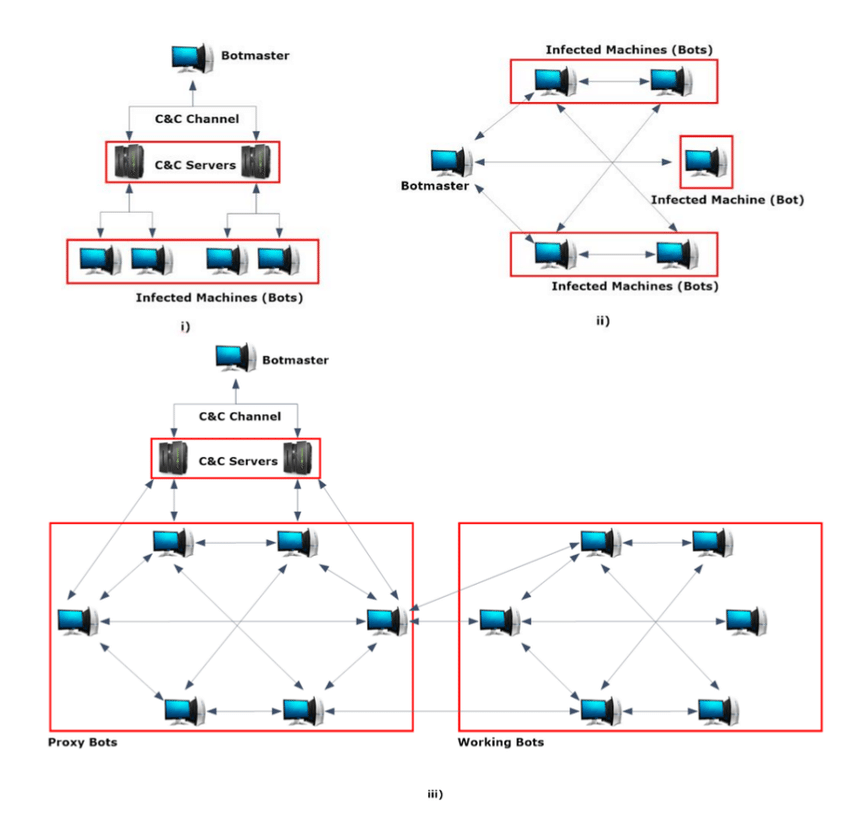
\includegraphics[scale=0.5]{figs/topologias.png}
\label{f.topologias}
\legend{\small Fonte: \cite{imagembotnets}.}
\end{figure}

As \textit{botnets} descentralizadas, por não possuírem uma estrutura central de comando, são mais difíceis de serem rastreadas e derrubadas, enquanto as centralizadas são mais suscetíveis a serem derrubadas, tendo em vista que se o Servidor de C\&C for desativado, a \textit{botnet} deixa de funcionar. \cite{feily2009survey}

Por outro lado, as \textit{botnets} centralizadas são muito mais confiáveis e eficientes na questão da comunicação, enquanto as P2P apresentam problemas de latência que acabam diminuindo o poder de seus ataques. Tendo isso em vista, as topologias centralizadas ainda são utilizadas pela sua facilidade de utilização e gerenciamento, além da baixa latência \cite{12d2f5d1eba245f7bc2acc7487941bd7}. Dentre estas, se destacam as que utilizam o protocolo IRC e HTTP.

O Protocolo \textit{Internet Relay Chat} foi desenvolvido para ser utilizado em aplicações de trocas de mensagens em grupo \cite{oikarinen1993internet}. Ele é baseado num modelo de cliente-servidor, onde um processo funciona como um ponto central, guardando o estado global de todos os outros clientes conectados a ele. Devido a um grande número de aplicações \textit{open-source} baseadas no protocolo IRC, sua implementação acaba sendo muito mais fácil, sendo esse o motivo pelo qual é o mais prevalente historicamente, e o motivo de ser o foco deste estudo. \cite{abu2006multifaceted}

O ciclo de vida de uma \textit{botnet}, segundo \cite{leonard2009framework}, pode ser descrito em quatro passos:

\begin{itemize}
    \item Infecção: nesta etapa, o \textit{botmaster} age infectando várias máquinas com \textit{malwares}, incorporando-as desta maneira à rede;
    \item Ambiente de Comando e Controle: depois de infectada, uma máquina estabele então uma conexão com o Servidor de C\&C, ficando à disposição do mestre para que quando ele desejar, possa enviar uma mensagem para o Servidor, e através deste a ordem é então repassada para todos os \textit{bots} conectados à sua rede;
    \item Ataque: depois que os \textit{bots} recebem as ordens, eles passam então a executar aquilo que foi determinado pela instrução enviada, como enviar \textit{e-mails} de \textit{spam}, por exemplo;
    \item Pós-Ataque: depois que o ataque foi concluído, alguns \textit{bots} podem ser descobertos, levando a uma remoção do vírus e consequentemente, a remoção da máquina da \textit{botnet}. Sendo assim, o foco do mestre é executar a manutenção da rede, e por fim focar no recrutamento de novas máquinas, ponto onde o ciclo recomeça.
\end{itemize}

Na área de detecção de botnets, têm se destacado muito por sua eficiência técnicas baseadas na mineração de dados, utilizando algoritmos de ML, como observado em \cite{feily2009survey}. A maioria destas técnicas de detecção costumam trabalhar com fluxos de redes, ao invés de pacotes isolados, devido ao fato dos primeiros apresentarem uma possibilidade muito maior de características a serem utilizadas \cite{beigi2014towards}. 

Muitos estudos têm sido feitos nos últimos anos com base nessas técnicas, explorando várias abordagens presentes na literatura de ML, variando desde a utilização de técnicas clássicas como por exemplo o algoritmo de Regressão Logística \cite{logregbot}, até o uso de técnicas mais recentes da área de \textit{Deep Learning}, através da implementação de Redes Neuras Artificiais Convolucionais, como estudado em \cite{rna1} e \cite{rna2}.

\section{Machine Learning}

\textit{Machine Learning} é uma subárea da IA que busca desenvolver algoritmos capazes de extrair conhecimento com base em dados, através da junção de conceitos de Estatística e Ciência da Computação \cite{James:2014:ISL:2517747}. 

Existem dois tipos principais de algoritmos de ML, os algoritmos supervisionados e não-supervisionados.

\subsection{Supervisionado e Não-supervisionado}

Na área de ML supervisionado, são fornecidos os dados de entrada e os dados de saída respectivos, e com base nestes, o algoritmo busca interpretar e buscar padrões nestes dados que possa diferenciá-los. 

Dentro do contexto de algoritmos de ML supervisionados, que é o foco deste trabalho, existem dois tipos de problema principais: Regressão e Classificação.

Problemas de Regressão são capazes de predizer variáveis quantitativas, ou seja, valores numéricos. Um exemplo seria encontrar o ganho anual de uma pessoa de acordo com a escolaridade, idade e local de residência. \cite{muller2017introduction} 

Já para o caso onde tenta-se predizer uma variável qualitativa, ou seja, encontrar a qual classe $C_{n}$ um certo item de entrada pertence, dado um conjunto de $n$ classes, têm-se um problema de Classificação. Para casos onde $n=2$, têm-se uma classificação binária, e quando $n>2$, uma classificação multi-classe.

Já em métodos não-supervisionados, as classes dos dados não são passadas ao algoritmo, de maneira que ele busca identificar padrões e relações entre eles, procurando alguma informação possa ser obtida delas. 

Para isso, utilizam-se principalmente as chamadas técnicas de clusterização, que buscam separar os dados em vários grupos de acordo com suas características observadas no conjunto de dados. \cite{muller2017introduction} 

\subsection{Fases de treinamento e teste}

Na área de ML costuma-se utilizar dois conjuntos de dados diferentes na fase de criação de modelos: conjunto de teste e conjunto de treino. O primeiro é utilizado pelo algoritmo para aprender as relações entre os dados, e o de teste para validar a sua eficiência.

Para que se obtenham esses conjuntos, uma prática comum é utilizar a técnica de \textit{Holdout}, que separa uma parte do conjunto de dados para que seja utilizada para teste, enquanto o resto é usado para treinar o modelo. Geralmente isso é definido através de uma proporção, como 70\% do conjunto para teste e 30\% para treino, por exemplo. \cite{van2010process}

Utilizando essa abordagem, espera-se observar que o modelo treinado seja generalizado, capaz de prever dados os quais nunca tenha trabalhado antes da maneira correta. No entanto, isto pode não ocorrer devido a:

\begin{itemize}
    \item \textit{Overfitting}: ocorre quando o modelo fica muito sensível a certas particularidades do conjunto de treinamento. Isto costuma ocorrer em modelos mais complexos que utilizam um número muito grande de características.
    \item \textit{Underfitting}: ocorre quando o modelo, por ser muito simples, não é capaz de aprender as características dos dados, e dessa maneira falha em apresentar os resultados esperados. 
\end{itemize}

O desafio na área de ML então é obter um modelo que esteja bem balanceado, não sendo nem muito simples nem muito complexo, de modo a evitar um dos problemas descritos acima. Para isto, podem-se utilizar várias técnicas, dentre elas se destacando o \textit{Cross Validation}, que buscam medir a generalização dos dados \cite{muller2017introduction}.

A técnica de CV baseada em k-folds consiste em separar o conjunto de treinos em k subconjuntos de tamanhos iguais, onde cada um será usado para treinar um modelo diferente . Estes modelos então são verificados alternando o conjunto de treino e utilizando os outros $k-1$ como teste, e a performance do algoritmo é obtida através da média das performances individuais. 

Algo importante de se notar também é a distribuição do número de amostras. De maneira geral, classificadores costumam ser muito mais efetivos quando trabalham com dados que se encontram balanceados, tendo sua efetividade diminuída caso contrário. \cite{yap2014application}

Neste contexto, podem ser aplicadas duas técnicas: \textit{Oversampling} e \textit{Undersampling}, que buscam aumentar ou diminuir, respectivamente, o número de amostras de uma classe específica de maneira a deixar o conjunto balanceado. A técnica de \textit{Oversampling} costuma ser mais trabalhosa por envolver a criação e adição de novos dados ao conjunto. 

Por fim, outro conceito importante para a generalização dos algoritmos é o dos hiper-parâmetros. Alguns algoritmos possuem parâmetros especiais que definem o seu desempenho e performance, e enquanto alguns algoritmos trabalham bem com seus valores padrão, para outros é necessário executar testes para encontrar os valores ótimos a serem passados. 

Neste contexto, utiliza-se a técnica de \textit{Grid Search}. Esta técnica consiste em testar todas as combinações possíveis de um certo conjunto de valores e verificar qual delas gera o melhor modelo possível \cite{bergstra2012random}.  É possível utilizá-la em conjunto com a técnica de CV para obter um nível de confiabilidade maior.

\subsection{Métricas}

Para se medir a eficiência de um algoritmo, pode-se classificar cada uma de suas predições dentro de quatro possibilidades: Verdadeiro Positivo (VP), Verdadeiro Negativo (VN), Falso Positivo (FP), Falso Negativo (FN). Estes dados são convenientemente agrupados para melhor visualização na chamada Matriz de Confusão. \cite{flach2003geometry}

\begin{figure}[h]
\caption{\small Exemplo de Matriz de Confusão.}
\centering
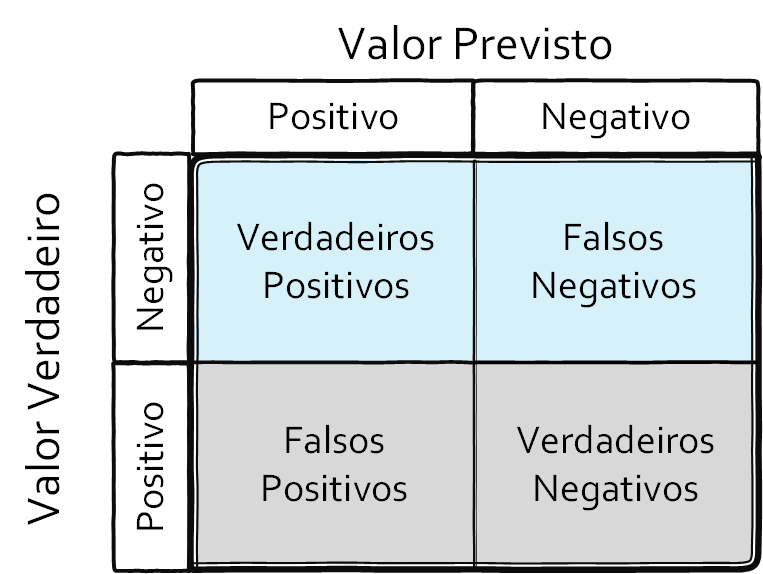
\includegraphics[scale=0.3]{figs/matrizconf.png}
\label{f.matriz-conf}
\legend{\small Fonte: \cite{matriz}.}
\end{figure}

A partir desses dados, é possível obter alguns valores que indicam a eficiência do algoritmo, os quais se destacam:

\begin{itemize}
    \item Precisão: $\frac{VP}{(VP + FP)}$
    \item Recall: $\frac{VP}{VP + FN}$
    \item F-score: $\frac{2 . Precisao . Recall}{(Precisao + Recall)}$
    \item Acurácia: $\frac{VP + VN}{VP + VN + FP + FN}$
    
\end{itemize}

\subsection{Algoritmos}

Nesta seção, serão apresentados os algoritmos da área de ML estudados para a execução deste trabalho.

\subsubsection{Naive Bayes}

Naive Bayes é um classe de algoritmos de ML que possuem sua fundação no Teorema de Bayes. Possui o nome \textit{Naive}, pois é baseado na suposição de que todas as características do problema são independentes umas das outras, algo que muito raramente acontece na grande maioria das aplicações do mundo real.

No entanto, apesar de sua suposição "inocente", classificadores NB são um dois mais eficientes e efetivos algoritmos da área de ML, sendo que se destacam de maneira maior na área de classificação de textos. \cite{zhang2004optimality}

Dada uma classe c, e um conjunto de características $F = x_{1},x_{2},...,xn$, a relação entre elas com base no Teorema de Bayes pode ser descrita da seguinte fórmula:

\begin{equation}
\label{e.bayes}
P(c,F)=\frac{P(F|c)P(c)}{P(F)},
\end{equation} e a suposição \textit{naive} de que todas as variáveis são independentes umas das outras implica que probabilidade de uma variável dado o valor da classe não depende do valor das outras variáveis do conjunto. Isso pode ser representado da seguinte forma:

\begin{equation}
\label{e.naive}
P(F,c)=P(x_{1},x_{2},...,x_{n}|c)=\Pi_{i=1}^n P(xi|y)
\end{equation} ou seja, a probabilidade do conjunto F sobre c pode ser representada pelo produto das probabilidades individuais de cada característica $x_{i}$ do conjunto sobre uma classe.

Sendo assim, é possível obter uma equação para Naive Bayes como se segue:

\begin{equation}
\label{eq_final}
r = arg max_{r}P(c)\Pi_{i=1}^n P(x_{i}|y)
\end{equation} que mostra que o rótulo de uma entrada r será atribuído verificando para qual valor de classe c é obtido uma maior probabilidade com base no conjunto de características do problema.

O que vai diferenciar os tipos de algoritmos de Naive Bayes é o modo como $ P(x_{i}|y)$ é calculado, ou seja, qual o tipo de distribuição que será usada. Estas podem ser Multinomial, Gaussiana ou Bernoulli \cite{Metsis06spamfiltering}. 

\subsubsection{Support Vector Machines}

O algoritmo de \textit{Support Vector Machines} foi criado na década de 90 por \cite{cortes1995support}, e desde então vem recebendo muita atenção da comunidade de ML por seu alto desempenho. Ele foi pensado inicialmente como um classificador binário, no entanto, muitas extensões foram desenvolvidas que permitem o uso da técnica para problemas de classificação de mais de uma classe e para regressão.

A ideia básica do SVM é encontrar um hiperplano ótimo que seja capaz de dividir os dados em duas regiões, de maneira que cada uma delas contenham dados de uma só classe. A equação geral de um hiperplano de dimensão $n$ é demonstrada a seguir:

\begin{equation}
\label{e.hyperplane}
\beta_{0} + \beta_{1}x_{1} + \beta_{2}x_{2} + ... = \beta_{n}x_{n} = 0
\end{equation} onde $x_{1},...,x_{n}$ representam as coordenadas de um certo ponto no ${\textrm I\!R}^{n}$ e $\beta_{1},...,\beta_{n}$ são constantes. 

Considerando que para um ponto $x_{n}$ que obedeça a igualdade, este ponto está localizado exatamente acima do hiperplano, o objetivo do algoritmo então é que, dado um problema que possui dados de duas classes $c_{1}$ e $c_{2}$, todos os pontos de uma destas tenha o seguinte comportamento  

\begin{equation}
\label{e.hyperplane-div1}
\beta_{0} + \beta_{1}x_{1} + \beta_{2}x_{2} + ... = \beta_{n}x_{n} > 0
\end{equation} enquanto para a outra classe seja observável que

\begin{equation}
\label{e.hyperplane-div2}
\beta_{0} + \beta_{1}x_{1} + \beta_{2}x_{2} + ... = \beta_{n}x_{n} < 0
\end{equation} ou seja, cada classe é encontrada somente em uma região, cada uma de um lado do hiperplano. Para definir a localização deste, busca-se um local onde a distância entre os pontos mais próximos do hiperplano de cada classe, neste contexto denominada margem, seja maximizado. Esta técnica é conhecida como \textit{Marginal Margins Classifier}
\cite{James:2014:ISL:2517747} A Figura \ref{f.hiperplano-svm} ilustra a ideia básica destes conceitos.

\begin{figure}[ht]
\caption{\small Hiperplanos no conceito de SVM.}
\centering
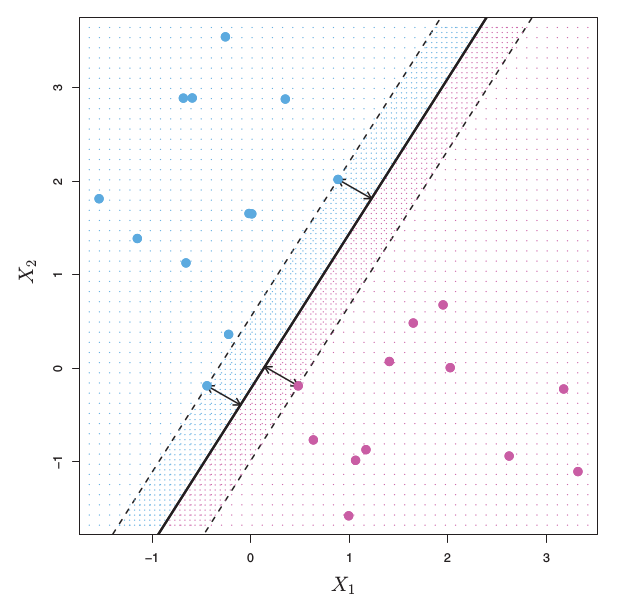
\includegraphics[scale=0.40]{figs/svm-plano.png}
\label{f.hiperplano-svm}
\legend{\small Fonte: \cite{James:2014:ISL:2517747}.}
\end{figure}

No entanto, um caso de dados totalmente capaz de ser separado linearmente é muito raro de ser obtido em uma situação real. Tendo isso em vista, pode ser utilizada uma abordagem diferente, \textit{Soft Margins Classifier} aonde é permitido que pontos estejam localizados não só na região da margem, mas inclusive do lado errado do hiperplano. 

Porém existem ainda os casos aonde os dados não possuem uma distribuição linear, e sendo assim não é possível estabeler um hiperplano entre as classes. Porém, estes dados podem ser separáveis em um espaço de maior dimensão, como demonstrado na Figura \ref{f.svm-transformacao} \cite{kim2013everything}. 

Depois de obtido o plano no espaço de maior dimensão, este pode ser projetado na dimensão anterior e assim se consegue um hiperplano divisor. Porém, o processo dessas transformações é muito caro computacionalmente, e neste contexto se faz útil a utilização do chamado \textit{Kernel Trick}.

\begin{figure}[ht]
\caption{\small Caso de uso de transformação em SVM.}
\centering
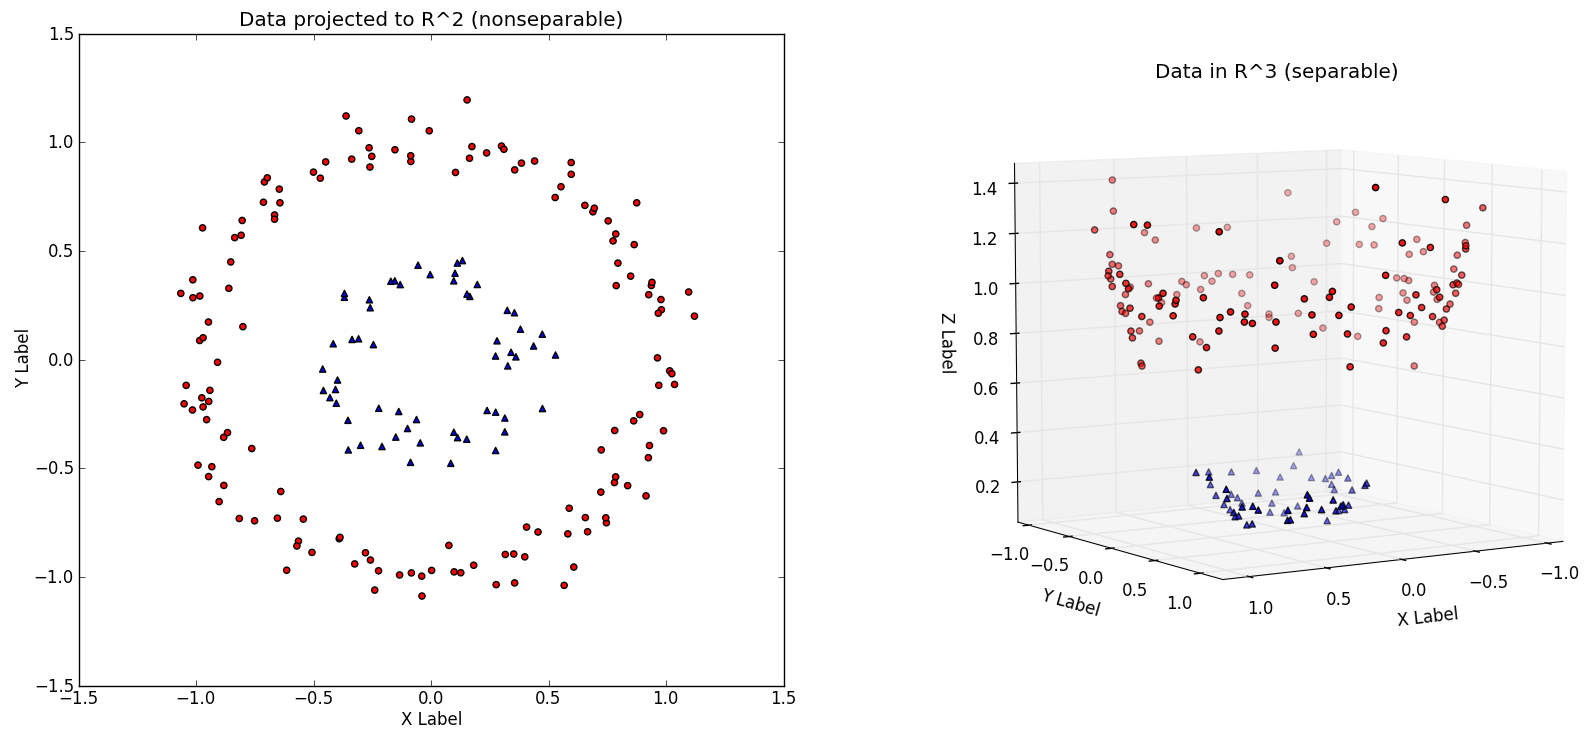
\includegraphics[scale=0.40]{figs/svm-2dto3d.png}
\label{f.svm-transformacao}
\legend{\small Fonte: \cite{kim2013everything}.}
\end{figure}

É possível observar através de comprovações matemáticas, que os resultados do algoritmo de SVM são obtidos através do produto escalar entre seus dados \cite{jordan2004kernel}. Neste contexto, são utilizadas as funções Kernel, que são capazes de calcular o produto escalar de dois vetores, representado por $<x,x'>$, no Rn em um espaço Rm, onde $m > n$, sendo assim capaz de calcular hiperplanos de maneira muito barata computacionalmente.

As funções Kernel mais utilizadas neste contexto são mostradas no Quadro \ref{t.kernels}.

\begin{quadro}[h]
\caption{Funções Kernel utilizadas em SVM.}
\centering
\begin{tabular}{|c p{5cm}|l p{5cm}}
\hline
\textbf{\small Nome} & \textbf{\small Função Kernel}\\\hline \hline
{\small Linear} & {\small $<x,x'>$}\\\hline
{\small Polinomial} & {\small $(\gamma<x,x'> + r)^{d}$}\\\hline
{\small Radial Basis Function} & {\small $\exp(-\gamma \parallel x - x' \parallel^{2})$}\\\hline
{\small Sigmoidal} & {\small $\tanh(\gamma<x,x'> + r)$}\\\hline
\end{tabular}
\legend{\small Fonte: Elaborado pelo Autor.}
\label{t.kernels}
\end{quadro}

Uma grande desvantagem do SVM é que eles exigem que seus hiper-parâmetros sejam muito bem otimizados para que ele tenha um bom desempenho, assim exigindo um estudo maior para ser utilizado. 

O Hiper-parâmetro C, constante de margens suaves, é comum a todos os Kernels e determina o peso da minimização dos erros no conjunto de treinamento. Além disso, como observado na Tabela \ref{t.kernels}, alguns Kernels possuem valores específicos que devem ser determinados como $\gamma$, $r$ e $d$ (\textit{degree}) \cite{lorena2007introduccao}.

\subsubsection{Árvores de Decisão}

Árvores de decisão, no contexto de ML, são métodos que se assemelham muito a fluxogramas, pois busca através de perguntas do tipo \textit{if-else} encontrar um certo resultado \cite{harrington2012machine}.

Para definir os testes e divisões, as árvores de decisão trabalham com uma abordagem denominada \textit{splitting}, onde de maneira recursiva os dados são divididos em regiões menores, de modo que eles fiquem de maneira mais dividida possível.

Uma árvore de decisão possui três tipos de nós:

\begin{itemize}
    \item Nó raiz: o nó inicial da árvore, por onde começa o processo de divisão;
    \item Nós de decisão: nós que contêm cada uma das decisões feitas pelo algoritmo, definem através de comparações qual o caminho a ser percorrido pela árvore;
    \item Nós folha: são os nós presentes no final da árvore. Eles indicam qual a classe que o algoritmo foi capaz de prever
\end{itemize}

Primeiramente, o algoritmo busca uma característica inicial para iniciar as divisões e ser o nó raíz, que no caso é a que pode dividir da melhor maneira possível o conjunto de dados de modo que as classes fiquem bem separadas, podendo inclusive dividir em mais do que duas regiões. Após a divisão, são adicionados nós de teste à árvore, e novas características são selecionadas para a divisão do próximo passo. A Figura \ref{f.arvore-iris} mostra o exemplo de uma árvore de decisão, baseada no conjunto de dados de flores iris.

\begin{figure}[h]
\caption{\small Exemplo de Árvore de Decisão.}
\centering
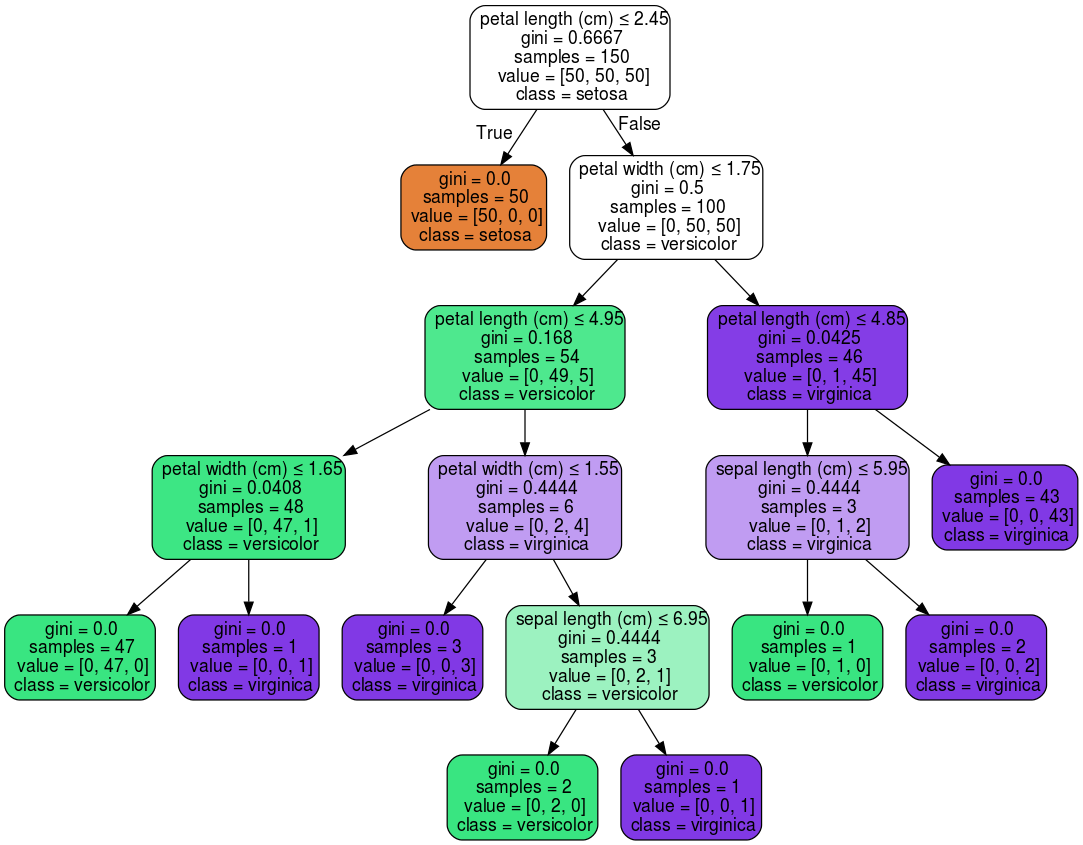
\includegraphics[scale=0.40]{figs/arvore-iris.png}
\label{f.arvore-iris}
\legend{\small Fonte: \cite{sklearn_api}.}
\end{figure}

Existem duas condições de parada para o algoritmos: as características possíveis para o problema se esgotarem, ou até que todas as instâncias das sub-regiões sejam pertencentes a uma mesma classe. \cite{James:2014:ISL:2517747}

Apesar deste método ser bem vantajoso por ser facilmente entendível e interpretável, infelizmente não são muito robustos por serem muito suscetíveis a perdas de precisão causadas por pequenas mudanças nas características, além de serem mais suscetíveis a \textit{overfitting}. 

\subsubsection{Florestas Aleatórias}

Florestas aleatórias é um método baseado em Árvores de Decisão. O algoritmo funciona com base em um número n, que determina quantas árvores são criadas, e para cada árvore n é selecionado de maneira aleatória um subconjunto de p características que esta árvore utilizará, considerando um número t de total de características. De maneira geral, o valor de p é calculado através de p = raiz quadrada de t. \cite{James:2014:ISL:2517747}

Este procedimento é muito eficiente, pois ao fazer com que as árvores sejam criadas com um número reduzido de características, elimina-se a possibilidade de que uma que seja muito mais forte do que as outras influencie tanto no resultado, de maneira que as árvores geradas sejam bem diferentes umas das outras e possuam um valor de variância mais alto entre elas. \cite{Breiman2001} 

Ao fim deste processo, as predições são feitas através de um sistema de votação. Os dados são passados por todas as árvores da floresta onde cada uma irá predizer uma classe, e enfim os votos serão contados e o resultado será definido pela classe com maior número de predições. 
Tomando como exemplo o caso de um sistema de classificação, que foi treinado por uma Floresta Aleatória de 100 árvores para separar suas entradas em duas classes X e Y. Cada entrada teria suas características processadas por todas as árvores e suas respectivas saídas obtidas. No caso de terem sido obtidos 60 predições de classe X e 40 predições de classe Y, essa entrada seria classificada como pertencente à classe X. A Figura \ref{f.random-forest} ilustra o funcionamento das Florestas Aleatórias.

\begin{figure}[h]
\caption{\small Funcionamento de Florestas Aleatórias.}
\centering
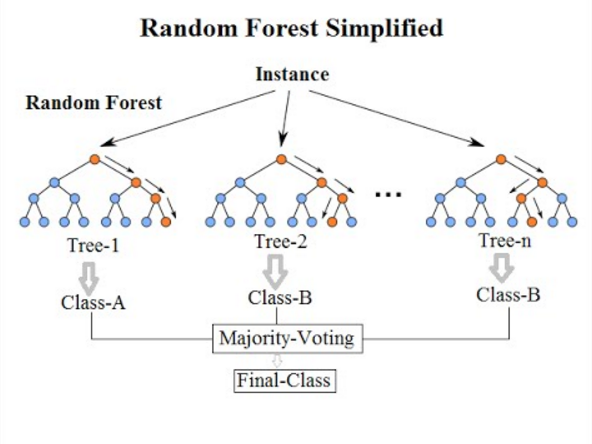
\includegraphics[scale=0.60]{figs/random-forests.png}
\label{f.random-forest}
\legend{\small Fonte: \cite{rfimagem}.}
\end{figure}

\subsubsection{AdaBoost}

AdaBoost, abreviação de \textit{Adaptive Boosting}, é um algoritmo formulado por \cite{FREUND1997119}, que busca melhorar a performance de outros classificadores. No contexto desse trabalho, será abordado a utilização deste algoritmo em conjunto com Árvores de Decisão.

O AdaBoost possui semelhanças com o algoritmo de Florestas Aleatórias, visto que ele busca trabalhar com um conjunto de classificadores de forma a obter um resultado mais confiável, porém se diferencia ao obter no final de seu processo, um modelo ao invés de utilizar a abordagem de votação.

O algoritmo funciona mantendo um valor de peso $w_{i}$ para cada dado do conjunto de treino passado para o algoritmo. Depois, são feitas várias iterações onde em cada uma é gerado um novo classificador fraco, que é o nome dado a um modelo que possui uma performance minimamente maior comparado a um algoritmo totalmente randômico, que possui acurácia próxima de 50 por cento.

É feita então uma predição com base neste algoritmo, e os pesos das variáveis são atualizados de acordo com o valor obtido pelo classificador, de maneira que se um dado foi classificado de maneira correta, seu peso diminui, e seu peso aumenta em caso contrário \cite{rojas2009adaboost}. Depois disso, o subconjunto utilizado pelo próximo classificador fraco é escolhido com base nos valores dos pesos. A Figura \ref{f.adaboost} ilustra o processo do algoritmo de AdaBoost.

\begin{figure}[h]
\caption{\small Funcionamento do AdaBoost.}
\centering
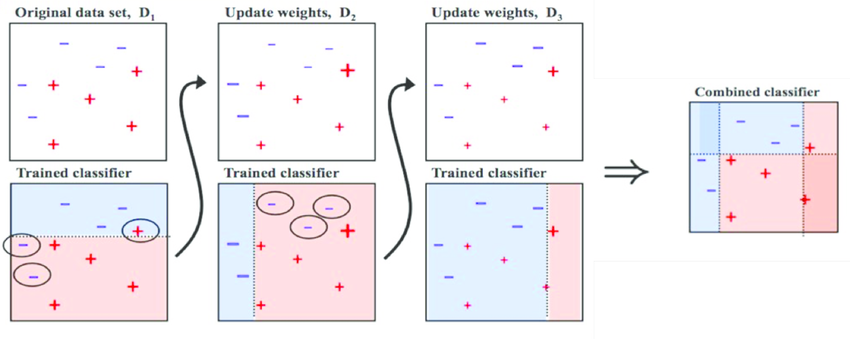
\includegraphics[scale=1.4]{figs/adaboost.png}
\label{f.adaboost}
\legend{\small Fonte: \cite{adaboost}.}
\end{figure}

Dessa maneira, o AdaBoost consegue favorecer em seus treinamentos o uso de variáveis que são mais difíceis de serem classificadas corretamente, o que faz dele muito eficiente em identificar \textit{outliers}. Ao final do processo, um modelo robusto é gerado com base nos passos anteriores dos classificadores fracos.

\subsubsection{Recursive Feature Elimination}

O RFE é um algoritmo recursivo que busca encontrar um subconjunto ótimo de características para um classificador específico, através do proceso de atribuição de um ranking de importância de cada uma delas.

O algoritmo começa sua execução com todas as características do conjunto passado, cria um modelo com base nelas, e calcula a importância de cada uma para a execução e performance do modelo. \cite{muller2017introduction} Depois disso, o algoritmo elimina a característica que teve o menor valor de importância e repete o processo recursivamente.

Ao final da execução, o algoritmo seleciona as $n$ características mais bem colocadas em seu ranking, obtendo assim o melhor conjunto possível, sendo $n$ um número pré-definido. 

\section{Revisão Bibliográfica}

Como base para este estudo, foram utilizados alguns artigos. O primeiro, \textit{Machine learning for identifying botnet network traffic} \cite{12d2f5d1eba245f7bc2acc7487941bd7}, faz um estudo comparativo entre vários estudos da área, separando-os de acordo com tipo de ML e protocolo estudado, e depois apresentando características de cada um. Desse estudo, foram obtidos os seguintes artigos como base:

\begin{quadro}[h]
\caption{Estudos da área utilizados como base para escolha dos classificadores.}
\centering
\begin{tabular}{|p{4cm}|p{5cm}|p{3cm}|}
\hline
\textbf{\small Autor(es)} & \textbf{\small Classificadores usados} & \textbf{\small{Características utilizadas}}\\\hline
{\small \cite{livadas2006usilng}} & {\small Árvores de Decisão,
Naive Bayes, 
Redes Bayesianas} & {\small 10}\\\hline
{\small \cite{strayer2008botnet}} & {\small Árvores de Decisão, Naive Bayes, Redes Bayesianas} & {\small 16}\\\hline
{\small \cite{masud2008flow}} & {\small Árvores de Decisão, Naive Bayes, Redes Bayesianas, SVM, Árvores de Decisão com Boosting} & {\small 20}\\\hline
\end{tabular}
\legend{Fonte: Elaborado pelo Autor.}
\label{t.articles}
\end{quadro}

De acordo com o Quadro \ref{t.articles}, foram obtidos os estimadores e características base deste trabalho, com algumas ressalvas. Nota-se que Redes Bayesianas se fazem presente em todos eles, no entanto as bibliotecas deste trabalho não possuem implementação deste algoritmo. Portanto, Florestas Aleatórias foi incluído como substituto, por também ter sido utilizado em estudos relacionados \cite{rna2}. 

Além disso, como não foi especificado nos trabalho quais técnicas de \textit{Boosted Decision Trees} e Naive Bayes foram utilizadas, optou-se pelo uso do AdaBoost e pelo teste de Naive Bayes Multinomial e Bernoulli, respectivamente.

O segundo estudo é o \textit{Towards Effective Feature Selection in Machine Learning-Based Botnet Detection Approaches} \cite{beigi2014towards}, que apresenta um estudo detalhado sobre as características de rede predominantes na área. Com base neste e nos estudos utilizados anteriormente, foram definidas quais delas seriam utilizadas. 

Em conjunto com estes, também foram observados outros estudos com base que também apresentaram a utilização dos mesmos conjuntos de características, como \cite{featureselection} e \cite{iscx1}.

Entre elas, têm-se:

\begin{itemize}
    \item IP/Port de Origem e Destino: Estas características são utilizadas para a identificação dos fluxos de rede maliciosos;
    \item Protocolo: utilizado principalmente para a etapa de filtragem de pacotes, diminuindo dessa maneira o volume de pacotes a serem processados pelo algoritmo. Por exemplo, no contexto de uma \textit{Botnet} que utiliza o protocolo UDP para comunicação, é possível então filtrar os fluxos para que contenham somente os que utilizam o mesmo;
    \item Duração: característica muito utilizada para identificação de todos os tipos de protocolos de \textit{Botnet}, tendo em vista que elas de maneira geral costumam ter dois tipos bem distintos de conexão, sendo uma conexão inicial bem rápida seguidas de sessões muito longas;
    \item Características de tamanho de fluxo: Nesta categoria, estão presentes o Total de Bytes/Bits/Pacotes , Bytes por Pacote e Tamanho Médio de \textit{Payload}. Estas características ajudam a distinguir o fluxo de uma \textit{Botnet} de um tráfico normal baseado no fato de que o tráfego de \textit{Botnets} costuma ser muito mais uniforme do que os outros, que apresentam comportamentos mais variados dependentes da aplicação;
    \item Características de tempo de conexão: Nesta categoria, estão presentes Média de pacotes/bits por segundo, Média e Variância do tempo entre transmissão de pacotes (IAT). São utilizadas pelos mesmos motivos das características de tamanho de fluxo, para distinguir pelo comportamento da rede os tráfegos de \textit{Botnet};
    \item IOPR/Porcentagem de pacotes enviados: IOPR representa a relação entre o número de pacotes que chegam sobre o número de pacotes que são enviados em uma conexão. Assim como a porcentagem de pacotes enviados, estas características estão ligadas a estudos que indicam que a relação entre pacotes enviados e recebidos em redes normais segue uma distribuição uniforme. Porém, como estudos como \cite{almgren2010tracking} indicam que em redes infectadas por agentes maliciosos esta relação costuma ser desbalanceada, e portanto, pode ser utilizada para identificação de \textit{Botnets}.
\end{itemize}


\chapter{Metodologia}
\label{c.metodologia}

\section{Ferramentas}
\label{s.ferramentas}

\subsection{Scikit-learn}
\label{ss.scikit}

O Scikit-learn é uma biblioteca open source de \textit{Machine Learning} na linguagem Python. O projeto iniciado em 2007 por David Cournapeau foi publicado oficialmente pela primeira vez em 2010, e desde então vem recebendo novas atualizações trimestrais, sendo que atualmente se encontra na versão 0.19.2. \cite{sklearn_api}

A ideia da biblioteca é oferecer acesso facilitado a várias ferramentas da área, que vão desde os algoritmos, supervisionados e não-supervisionados, até outras funcionalidades como transformadores de dados (Por exemplo, o módulo de Principal Component Analysis, e TfIdf para Processamento de Linguagem Natural) e ferramentas gerais como o Grid Search e Pipeline. \cite{scikit-learn}

A biblioteca não apresenta interface de linha de comando ou interface gráfica, sendo que todo seu funcionamento se dá através de chamadas de funções Python. 

Todas as classes da bibliotecas são construídas com base no mesmo padrão de interface básico, o que facilita muito o seu uso. Cada estimador possui um método 'fit' onde são passados os dados para que seja feito o treinamento, e um método 'predict' que executa as predições com base no modelo treinado no passo anterior. Além disso, todos os hiperparâmetros dos métodos são acessíveis e modificáveis através do seu respectivo construtor de classe.


Na figura \ref{f.exemplo-scikit} é demonstrado um exemplo de utilização da biblioteca para a execução do modelo de Regressão Linear.

\begin{figure}[h]
\caption{\small Exemplo de utilização do Scikit.}
\centering
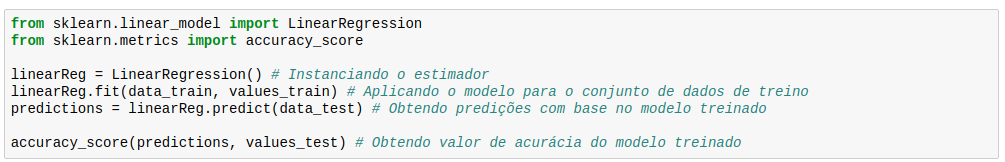
\includegraphics[scale=0.55]{figs/exemplo-scikit.png}
\label{f.exemplo-scikit}
\legend{\small Fonte: Elaborada pelo autor.}
\end{figure}


\subsection{Numpy}
\label{ss.numpy}

O NumPy é uma biblioteca, integrante do conjunto Scipy, feita em cima da biblioteca Numeric. Seu objetivo é fornecer várias funções e estruturas de dados que possam facilitar o uso da linguagem Python em um contexto científico. Teve sua primeira versão lançada em 2005, e atualmente se encontra na versão 1.15.1. \cite{numpy}

Algumas de suas funcionalidades são:

\begin{itemize}
  \item  Um poderoso objeto vetor de N-dimensões (denominado Numpy Array);
  \item Métodos para se trabalhar com vetores de maneiras mais sofisticadas;
  \item Funções de álgebra linear, transformações de Fourier e ferramentas para trabalhar com numeros aleatorios;
  \item Ferramentas de integração para códigos em Fortran e C/C++;
\end{itemize}

O NumPy se destaca por ser a base de várias outras bibliotecas científicas do Python, como o próprio Scikit que utiliza as estruturas de Numpy Array para seus cálculos.  

\subsection{Pandas}
\label{ss.pandas}

O Pandas é uma biblioteca que busca suprir uma demanda que a linguagem Python não tem por padrão, através de uma poderosa e robusta estrutura para se trabalhar com uma grande quantidade de dados estruturados, muito utilizados nas áreas de Estatística, Mercado Financeiro, Data Science, entre outros. \cite{pandas-article} O Pandas se destaca por ser baseado no NumPy, sendo assim muito facilmente integrado com todas as outras bibliotecas de ML em Python, e também por ser muito rápido e eficiente.

O Pandas apresenta duas estruturas de dados principais, \textit{Series} e \textit{Data Frames}, sendo a primeira uni-dimensional e a segunda bi-dimensional. Dentre essas duas se destaca o \textit{Data Frame}, similar ao \textit{data.frame} que está presente nativamente para a linguagem R, porém com algumas melhorias. A figura \ref{f.exemplo-pandas} ilustra um exemplo de uso desta estrutura.

Algumas das principais funções do Pandas são:

\begin{itemize}
    \item Fácil manipulação de dados nulos;
    \item Várias opções para leitura de arquivos, como por exemplo tabelas Excel, CSV, tabelas de Bancos de Dados, além de leitura de dados estruturados em arquivos HTML
    \item Inserção e remoção de colunas;
    \item Redimensionamento e obtenção de subsets;
    \item Muitos métodos utilizados no contexto de Bancos de Dados, como merge, join e groupby.
\end{itemize}

\begin{figure}[h]
\caption{\small Exemplo de utilização do Pandas.}
\centering
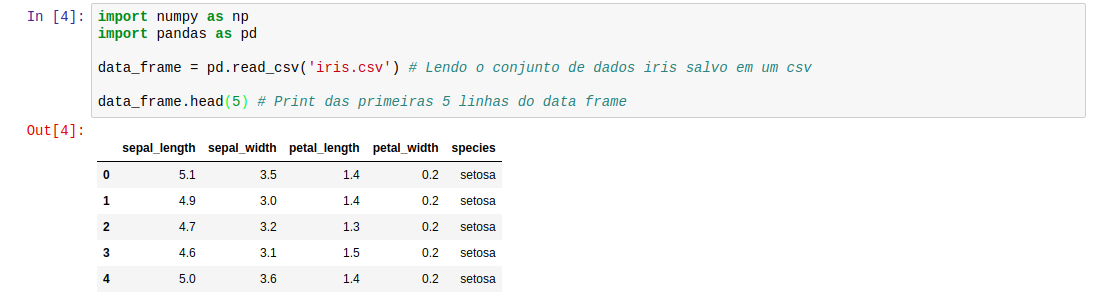
\includegraphics[scale=0.40]{figs/exemplo-pandas.png}
\label{f.exemplo-pandas}
\legend{\small Fonte: Elaborada pelo autor.}
\end{figure}

\subsection{Matplotlib}
\label{ss.matplotlib}

Matplotlib é uma biblioteca para criação de visualizações 2D em Python, que começou a ser desenvolvida em 2003 por John D. Hunter. O intuito da biblioteca era atender alguns requisitos, entre eles ser possível de ser integrado a uma interface gráfica, funcionar em diversas plataformas, oferecer suportes para publicações e funcionar em aplicações interativas. \cite{matplotlib}

O Matplotlib funciona com uma inteface similar ao do MATLAB, através do módulo pyplot. Com ele, é possível em poucas linhas ser capaz de gerar histogramas, gráficos de barra, gráficos de dispersão, entre outros.  A figura \ref{f.exemplo-matplotlib} demonstra a geração de m gráfico utilizando a biblioteca.

Além disso, os gráficos são altamente customizáveis, oferecendo controle total de elementos como estilos de linha, propriedades dos eixos, etc.

\begin{figure}[h]
\caption{\small Exemplo de utilização do Matplotlib.}
\centering
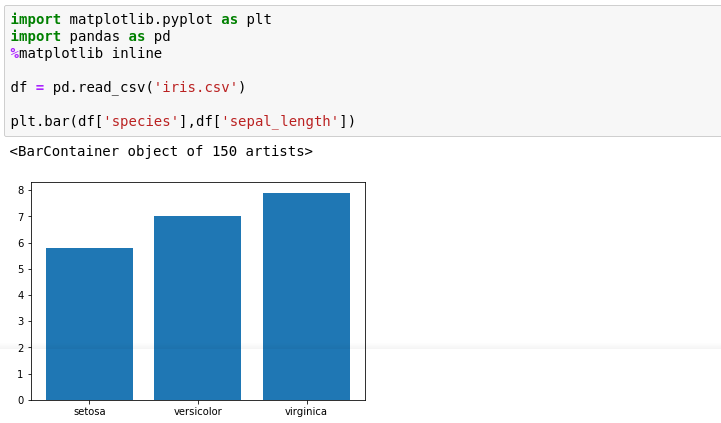
\includegraphics[scale=2]{figs/exemplo-pyplot.png}
\label{f.exemplo-matplotlib}
\legend{\small Fonte: Elaborada pelo autor.}
\end{figure}

\subsection{Seaborn}
\label{ss.seaborn}

O Seaborn é uma biblioteca Python, que funciona como um \textit{wrapper} para o Matplotlib. Ele busca simplificar ainda mais a geração de gráficos, oferecendo uma interface ainda mais simplificada que permite com que visualizações sejam geradas com apenas uma linha de código, como demonstrado na figura \ref{f.exemplo-seaborn}. Ele incorpora alguns tipos de gráficos mais avançados como Gráficos de Calor e Gráficos de violino, e também por padrão customiza os gráficos de uma maneira mais elegante, mesmo que eles tenham sido gerados usando somente o Matplotlib.

Todas as customizações são feitas através de parâmetros de função, e além disso é possível utilizar chamadas da biblioteca do Matplotlib para maiores customizações.

Além disso, o Seaborn traz em sua biblioteca um conjunto de \textit{datasets}, o que facilita na hora de se estudar as possibilidades de visualizações e entender relações entre variáveis.

\begin{figure}[h]
\caption{\small Exemplo de utilização do Seaborn.}
\centering
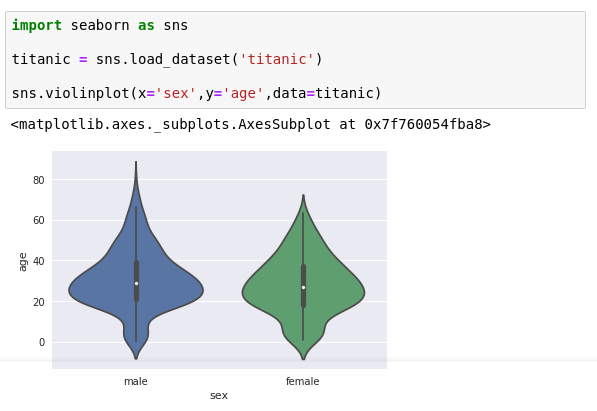
\includegraphics[scale=2.5]{figs/exemplo-seaborn.png}
\label{f.exemplo-seaborn}
\legend{\small Fonte: Elaborada pelo autor.}
\end{figure}

\subsection{Jupyter Notebook}
\label{ss.jupyter}

O Jupyter Notebook é uma aplicação \textit{web open-source}, que permite a criação de documentos, denominados Notebooks, que contenham códigos, equações, visualizações e textos explicativos. Iniciado em 2014, foi construído com base no projeto IPython, porém hoje já apresenta suporte para mais de 50 linguagens que variam de C++ até Bash. 

Um Notebook pode ser pensado como uma evolução dos consoles do tipo REPL (Read Evaluate Print Loop), que permitem com que comandos fossem inseridos de maneira interativa e seus respectivos outputs pudessem ser visualizados em tempo real, como observado pelo uso da ferramenta IPython na Figura \ref{f.exemplo-ipython}. O grande diferencial é que os arquivos do Jupyter permitem que as saídas de códigos sejam mais do que simples textos, apresentando suporte para imagens, controles e gráficos interativos e equações matemáticas formatadas. \cite{Kluyver:2016aa} 

\begin{figure}[h]
\caption{\small Exemplo de utilização do IPython.}
\centering
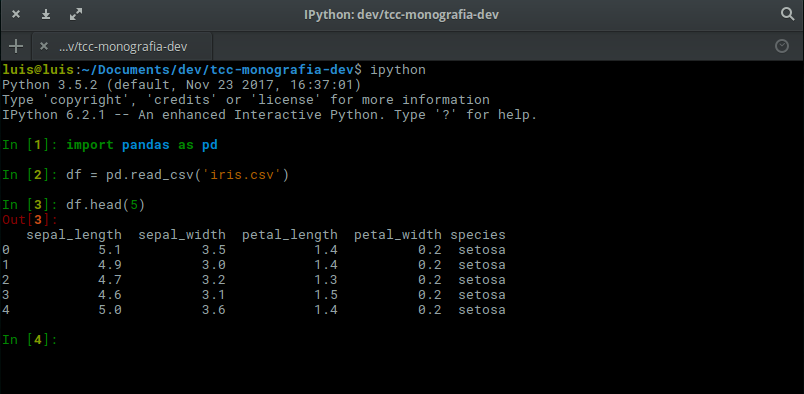
\includegraphics[scale=0.40]{figs/exemplo-ipython.png}
\label{f.exemplo-ipython}
\legend{\small Fonte: Elaborada pelo autor.}
\end{figure}

Os Notebooks foram pensados com o ambiente científico em mente, permitindo com que seja muito fácil visualizar e analisar dados facilitando o processo de desenvolvimento, assim como o posterior compartilhamento e publicação de modelos, tendo em vista que uma pessoa é capaz de não só visualizar todo o processo de criação do modelo assim como seus outputs e quaisquer textos de explicação adicionados pelo autor, mas também ser capaz de reproduzí-los em seu próprio ambiente simplesmente executando os códigos novamente.

Além disso, existem várias ferramentas que fazem com que o compartilhamento e acesso de Notebooks seja facilitado. Exemplos são o nbconvert, que converte o arquivo para os formatos HTML, PDF e LaTex, e o nbviewer que permite que \textit{Notebooks} hospedados na internet sejam visualizados no navegador sem necessidade de \textit{download}.

A execução do Jupyter se dá pela linha de comando, no diretório onde os arquivos estão presentes. Depois de executado, uma interface será aberta no navegador permitindo com que os arquivos sejam abertos e editados.

% \begin{figure}[h]
% \caption{\small Exemplo de execução do Jupyter no ambiente local.}
% \centering
% 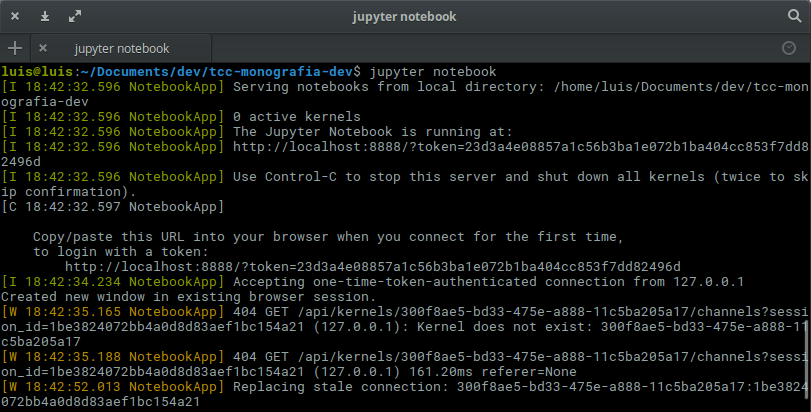
\includegraphics[scale=0.40]{figs/exemplo-jupyterutil.png}
% \label{f.exemplo-jupyterlocal}
% \legend{\small Fonte: Elaborada pelo autor.}
% \end{figure}

% \begin{figure}[h]
% \caption{\small Demonstração de interface do Jupyter.}
% \centering
% 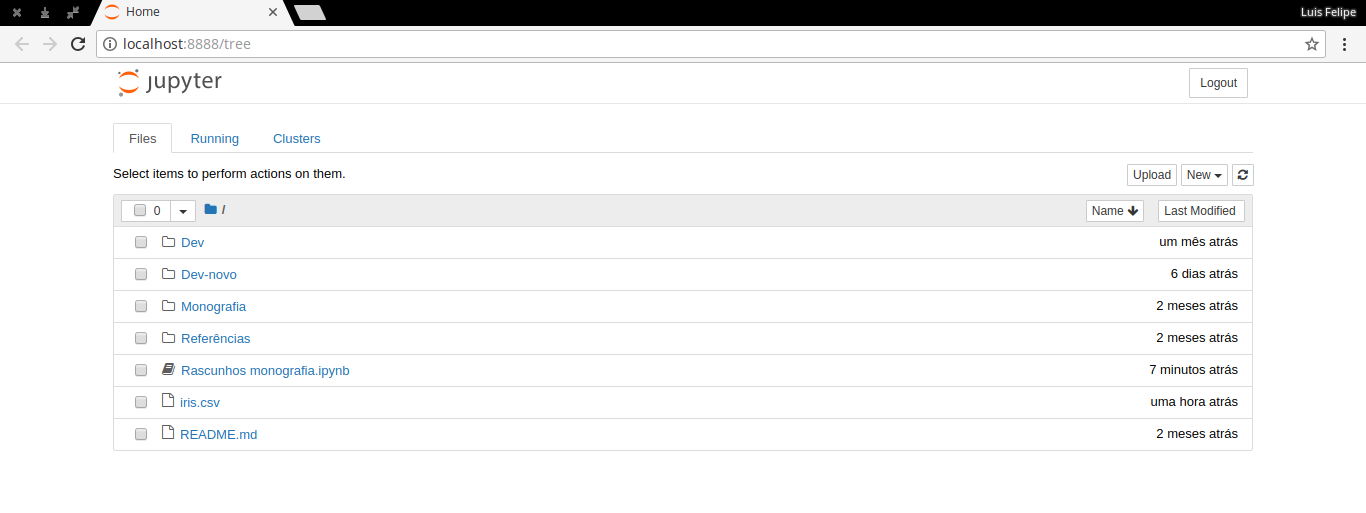
\includegraphics[scale=0.25]{figs/exemplo-jupyterinterface1.png}
% \label{f.exemplo-jupyterinterface}
% \legend{\small Fonte: Elaborada pelo autor.}
% \end{figure}

\chapter{Desenvolvimento}
\label{c.desenvolvimento}

\section{Base de dados}

Para este trabalho foi utilizada uma base de dados fornecida pela \textit{University of New Brunswick} \cite{unbdataset}. Esta base vem sendo utilizada em vários estudos recentes da área, como \cite{iscx1} e \cite{rna1}, e portanto sua utilização é de extrema relevância. Foram fornecidos três arquivos no formato PCAP, sendo um voltado para a fase de treinamento e dois para testes. No entanto, os arquivos de teste apresentaram problemas, com ambos não podendo ser processados pelo programa.

Um deles apresentava problemas de desordenamento dos pacotes, que ao tentar ser resolvido levou a uma descaracterização dos dados, como por exemplo valores de duração negativos, algo que não é possível por se tratar de uma medida de tempo. Já o segundo apresentou problemas de corrompimento, que também impediram seu processamento.

Sendo assim, todo o desenvolvimento deste trabalho, assim como seus resultados, serão baseados somente no conjunto de treino fornecido, utilizando a técnica de \textit{Hold-out} explicada anteriormente.

\section{Geração de fluxos de rede}
\label{d.fluxo}

Para que os estimadores pudessem trabalhar no conjunto de dados, foi preciso primeiro passar os arquivos de pacotes por um gerador de fluxos bidirecionais, um programa capaz de analisar todos os pacotes e extrair características dos fluxos de rede presentes nele.

Para este fim, foi utilizado o programa \textit{flowtbag}, uma ferramenta \textit{open-source} desenvolvida na linguagem \textit{Go}, disponível no \textit{GitHub} \cite{flowtbag}. A interface de utilização do programa se dá através da linha de comando, onde são passados o caminho para o arquivo de pacotes a ser analisado, e o caminho para onde o arquivo final, no formato CSV, deve ser salvo.

\begin{figure}[h]
\caption{\small Gerando arquivo de fluxos bidirecionais com a biblioteca \textit{flowtbag}.}
\centering
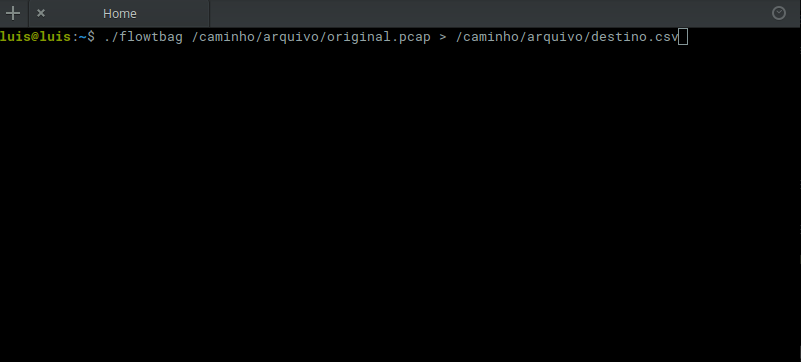
\includegraphics[scale=0.50]{figs/exemplo-flowtbag.png}
\label{f.exemplo-flowtbag}
\legend{\small Fonte: Elaborada pelo autor.}
\end{figure}

O arquivo CSV que o programa cria contém uma tabela onde as linhas representam cada fluxo de rede, e as colunas representam as características extraídas. Ao todo são 44 características,sendo que as cinco primeiras são as que definem um fluxo: IP de origem, IP de destino, Porta de origem, Porta de destino, e Protocolo.

Além das acima citadas, se fazem presentes no conjunto:

\begin{itemize}
    \item Total de Bytes;
    \item Total de Pacotes;
    \item Total de bytes alocados para cabeçalhos de pacote;
    \item Mínimo/Máximo/Média/Desvio Padrão da média de: menor pacote enviado, IAT, tempo ativo, tempo ocioso, ocorrências da flag \textit{Push}, ocorrências da flag \textit{Urgent};
\end{itemize}

As características de fluxo acima, com exceção de tempo ativo e tempo ocioso, são dividas em dois tipos: \textit{forward}, indica os valores correspondentes ao que foi enviado do IP de origem ao IP de destino, e \textit{backwards} indica o contrário, ou seja, o que o destinatário enviou a quem iniciou a conexão. Por exemplo, o número de pacotes trocados durante o fluxo é representado por dois valores, \textit{totalfpackets} e \textit{totalbpackets}, onde o primeiro indica quantos pacotes foram transmitido na direção \textit{forward} e o segundo na direção \textit{backward}. 

\section{Processamento de dados}

Depois de gerados o arquivo CSV, foi preciso fazer uma análise e processamento dos dados de forma que eles fossem usados pelos estimador. Para isto, foram utilizadas varias funcionalidades da biblioteca Pandas.

O programa gerador utilizado faz o processamento de conexões que utilizam o protocolo TCP e UDP, porém como o foco do projeto é analisar o fluxo de botnets do protocolo IRC, que por sua vez utilizam o protocolo TCP para transporte \cite{livadas2006usilng}, como explicado anteriormente, foi feita uma filtragem para que somente os protocolos desse tipo fossem mantidos na base de dados. 

Os fluxos de protocolo TCP eram representados pelo número 6, enquanto o número 17 representava os fluxos UDP. Dessa maneira, foi necessário somente filtar os fluxos com número de protocolo igual a 6.

Depois de eliminado os fluxos que não iriam ser utilizados, foi feita a rotulação dos dados, que consiste em atribuir para cada uma das linhas da tabela um valor que indica se aquele fluxo é de botnet ou não. Para essa tarefa, foram utilizados dois recursos: uma lista de IP's fornecida juntamente com a base de dados que informa o IP usado pelas botnets, e uma tabela pertencente ao estudo desenvolvido em conjunto com a base, que informa quais são as botnets presentes em cada conjunto.

Com essas informações, foi possível então desenvolver um método que iterasse por toda a tabela verificando se os IPs dos fluxos correspondiam aqueles dos ataques. Em caso positivo, era atribuído o valor 1, e 0 caso contrário.

\begin{figure}[h]
\caption{\small Rotulação dos fluxos.}
\centering
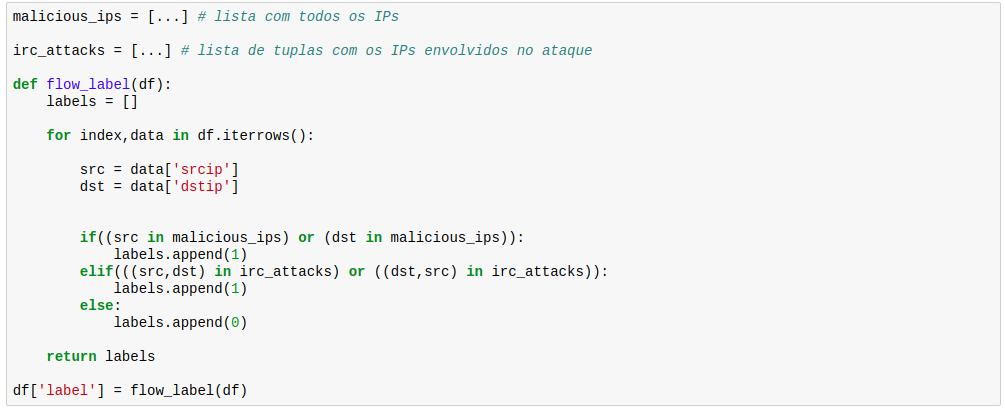
\includegraphics[scale=0.40]{figs/rotulacao-dados.png}
\label{f.rotulacao-dados}
\legend{\small Fonte: Elaborada pelo autor.}
\end{figure}

Além disso, foram também eliminados todos os fluxos de Botnets que não fossem do protocolo IRC, evitando assim com que houvesse interferência dessas informações nos resultados, tendo em vista que apesar de utilizarem protocolos diferentes, as redes ainda podem compartilhar certos tipos de comportamentos gerais, o que poderia acarretar em predições equivocadas.

Por fim, foi observado que a distribuição de fluxos por classe estava desbalanceada, com 86695 fluxos da classe 0 e somente 6379 da classe 1. Como os classificadores costumar trabalhar melhor com distribuições de dados balanceadas,foi aplicada a técnica do \textit{Undersampling}, diminuindo o número de amostras da classe 0 para o mesmo número de amostras da classe 1.

Foi necessário também criar algumas colunas de dados que não foram geradas automaticamente pelo programa. Como citado na seção anterior, o programa gerador divide as características em dois tipos, \textit{forward} e \textit{backward}, o que permite uma maior flexibilidade ao se trabalhar com os dados, porém exige que alguns cálculos sejam feitos para se gerar certas características mais gerais.

Foi preciso então, criar métodos capazes de trabalhar com os valores presentes para gerar alguns dados que foram utilizados em pesquisas anteriores da área. A tabela 1 mostra quais são essas características e como elas foram calculadas:

\begin{table}[ht]
\centering
\begin{tabular}{|c p{10cm}|l p{10cm}}
\hline
\textbf{\small Característica} & \textbf{\small Fórmula geradora}\\\hline \hline
{\small Total de Bytes} & {\small Soma dos bytes enviados em ambas as direções}\\\hline
{\small Total de pacotes} & {\small Soma dos pacotes enviados em ambas as direções}\\\hline
{\small Total de Bits} & {\small Número total de bytes multiplicado por 8 (1 byte = 8 bits)}\\\hline
{\small Bytes por pacote} & {\small Razão entre o Total de Bytes e Total de pacotes}\\\hline
{\small Bytes por segundo} & {\small Total de bits dividido pela duração do fluxo}\\\hline
{\small Pacotes por segundo} & {\small Total de pacotes dividido pela duração do fluxo}\\\hline
{\small Média de IAT} & {\small Média da soma dos valores IAT médios}\\\hline
{\small Bytes por segundo} & {\small Total de bits dividido pela duração do fluxo}\\\hline
{\small Média de variância de IAT} & {\small Média dos desvio padrão de IAT ao quadrado}\\\hline
{\small Porcentagem de pacotes enviados} & {\small Razão entre o número de pacotes enviado na direção \textit{forward} e o número total de pacotes do fluxo}\\\hline
{\small IOPR} & {\small Razão entre a quantidade de pacotes na direção \textit{backward} sobre a quantidade da direção \textit{forward}}\\\hline
{\small Média de tamanho de payload} & {\small Número de bytes total do fluxo menos a soma de bytes dos headers em ambas as direções, depois dividido pelo número de pacotes}\\\hline
\end{tabular}
\caption{Fórmulas utilizadas para geração de características.}
\label{t.caracteristicas-geradas}
\end{table}

\begin{figure}[h]
\caption{\small Exemplo de geração de colunas.}
\centering
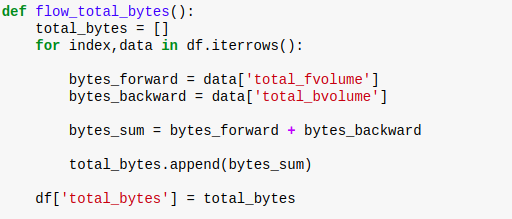
\includegraphics[scale=0.40]{figs/exemplo-geracao-coluna.png}
\label{f.exemplo-colunas}
\legend{\small Fonte: Elaborada pelo autor.}
\end{figure}

A figura \ref{f.exemplo-colunas} mostra o processo básico para a geração dessas colunas, utilizando como exemplo a coluna "Total de bytes". As linhas da tabela inteira são percorridas, as características necessárias para a geração são obtidas, as operações efetuadas e o resultado é adicionado para uma lista. Por fim, essa lista era adicionada no conjunto de dados como uma nova coluna. O processo é o mesmo para todas as outras características, alterando-se somente os cálculos e valores utilizados.

Por fim, foram removidas algumas colunas em que todos os valores eram 0, ou seja, dados que o gerador não foi capaz de obter nenhuma informação no conjunto de dados. Estas colunas foram as seguintes: Desvio padrão de tempo ativo de conexão, tempo mínimo de ociosidade na conexão,média de tempo de ociosidade na conexão, tempo máximo de ociosidade na conexão, desvio padrão do tempo de ociosidade na conexão, número de vezes em que a \textit{flag Urgent} foi enviada da origem para o destino, e número de vezes em que a \textit{flag Urgent}  foi enviada do destino para a origem.

Junto com estas, também foram removidas colunas que não são relevantes para os algoritmos, IP/Porta de origem e de destino e protocolo, que apesar de terem sido muito úteis para a rotulação e filtragem, não serão utilizados para a tarefa de classificação, entre outras.

\begin{figure}[h]
\caption{\small Removendo colunas nulas e desnecessárias para a classificação do conjunto.}
\centering
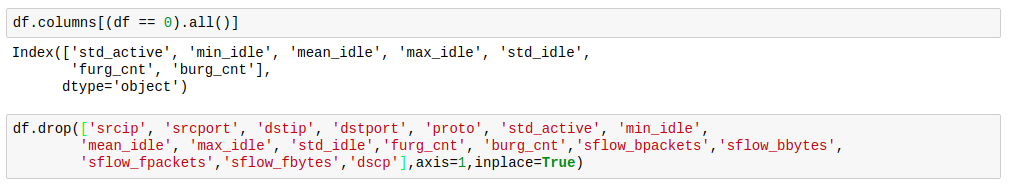
\includegraphics[scale=0.40]{figs/drop-colunas.png}
\label{f.drop-colunas}
\legend{\small Fonte: Elaborada pelo autor.}
\end{figure}

\section{Execução dos algoritmos}

Com os dados preparados, é possível então usá-los para treinar os algoritmos. Contando todas as colunas válidas do gerador e as características geradas manualmente e desconsiderando a coluna de rótulos, têm-se 39 colunas de características.

No entanto, não é viável executar os estimadores com todas, mas sim tentar encontrar um subconjunto destas que melhor caracterize o problema. Para este fim, foram aplicadas duas abordagens:

\begin{itemize}
    \item Busca de força bruta com base em dados de pesquisas anteriores: foram utilizadas somente as características presentes em trabalhos da área, e através de uma pesquisa de força bruta rodar todas as combinações delas com todos os algoritmos e assim desta maneira encontrar o melhor conjunto de características para cada classificador;

    \item Busca utilizando um algoritmo específico de seleção de características: o Scikit possui vários algoritmos para seleção de características, que buscam encontrar dado um conjunto a melhor combinação. Para este trabalho, será utilizado o RFE no conjunto inteiro de dados, tanto os do gerador de fluxo quanto os criados com base em estudos anteriores. 
\end{itemize}

\subsection{Busca de força bruta com base em dados de pesquisas anteriores}
\label{ss.dados-hist}

Para essa primeira abordagem, a ideia era testar todas os subconjuntos possíveis de características com todos os estimadores, e verificar qual combinação de características seria melhor com cada um deles.

Para obter as combinações de características do conjunto, foi utilizada a biblioteca \textit{itertools} do Python. A figura x mostra o processo de geração dos subconjuntos, aonde foi definido um numero mínimo de características por conjunto de 4. O resultado gerado é uma lista contendo todas as combinações. Ao fim do processo, foram geradas 1816 possibilidades.

\begin{figure}[h]
\caption{\small Gerando combinações com a biblioteca \textit{itertools}.}
\centering
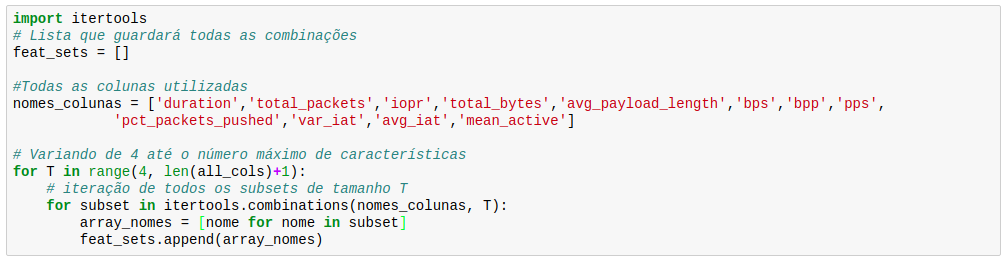
\includegraphics[scale=0.40]{figs/exemplo-itertools.png}
\label{f.exemplo-itertools}
\legend{\small Fonte: Elaborada pelo autor.}
\end{figure}

Depois, todas as combinações foram processadas por todos os estimadores, e as acurácias dos modelos obtidas. Foram criados vetores contendo instâncias de todos os estimadores a serem utilizados no trabalho, e depois este era percorrido, de maneira que a cada iteração o modelo fosse treinado e uma predição fosse obtida, salvando em uma tabela a acurácia e qual conjunto de dados foi usado. A figura x mostra o método utilizado para este processo. 

Ao fim deste processo, foi possível filtrar os dados da tabela pelas maiores acurácias de cada estimador, e assim encontrar o subconjunto ótimo para este, assim como a acurácia obtida.

\subsection{Utilizando o algoritmo Recursive Feature Elimination}
\label{ss.dados-rfe}

A ideia desta abordagem é utilizar o algoritmo RFE em todos o conjunto de dados, e dessa maneira observar quão eficaz são os dados utilizadas historicamente na área na tarefa de classificação, e também identificar se algumas das fornecidas pelo gerador são eficazes nesse processo, através do processo de observação das características escolhidas pelo algoritmo. 

Além disso, outro ponto dessa abordagem é verificar se as características utilizadas nos estudos anteriores possuem grande representatividade dado todo o conjunto de características, ou seja, se elas serão escolhidas pelo algoritmo.

O Scikit implementa o RFE em conjunto com a técnica de CV, para todos os números possíveis de parâmetros. Dessa maneira, é possível identificar não só um número fixo de características mas também encontrar qual o número ideal. Para utilizá-lo, passa-se como argumento uma instância do classificador desejado, e depois aplica-se a função \textit{fit} com um conjunto de treino, para que ele encontre o subconjunto ótimo.

Depois de encontrado, é possível acessar tanto o estimador quanto as características do conjunto de maneira ranqueada. Todas as características escolhidas são atribuídas o valor 1, e dessa maneira é possível tanto definir quais as características ótimas quanto já executar predições com o estimador que a estrutura fornece.  

\subsection{Otimização de Hiper-parâmetros}

Obtidos os melhores conjuntos de características para todos os estimadores utilizando as duas abordagens, o último passo a ser feito nesta etapa é aplicar a técnica de \textit{Grid Search} para otimizar hiper-parâmetros no algoritmo de SVM, que como explicado anteriormente na seção \ref{c.fundamentacao} é muito depende da otimização de seus hiper-parâmetros para obter melhores resultados.

O Scikit implementa a tecnica de \textit{Grid Search} em conjunto com o CV. A interface de utilização é muito parecida com a de um estimador normal, com a diferença de que deve ser passado também um dicionário com os parâmetros que serão testados e seus respectivos valores.

\begin{figure}[h]
\caption{\small Utilização do \textit{Grid Search} no Scikit.}
\centering
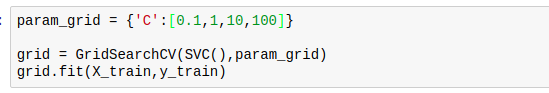
\includegraphics[scale=0.80]{figs/gridsearch.png}
\label{f.exemplo-gridsearch}
\legend{\small Fonte: Elaborada pelo autor.}
\end{figure}

Foram testados os Kernels Linear, RBF e Sigmoidal. Foram feitas tentativas de cálculo com o Kernel Polinomial, no entanto foram apresentados problemas de execução específicos que impediram a obtenção de resultados.

Foram testados os seguintes valores:

\begin{itemize}
    \item C: {0.1,1,10,100};
    \item $\gamma$: {0.0001,0.001,0.01,0.1,1};
    \item Coeficiente $r$, específico do Kernel Sigmoidal: {-1,0,1}.
\end{itemize}


\chapter{Resultados}
\label{c.resultados}

\section{Performance dos Classificadores}

As tabelas e gráficos a seguir mostram os resultados que foram obtidos na fase de Desenvolvimento. Nas tabelas \ref{r.t1} e \ref{r.t2}, constam os números de características e os valores de acurácia obtidos pelos classificadores ótimos encontrados tanto na abordagem de força bruta quanto na abordagem do RFE, respectivamente. Depois, são apresentados os gráficos \ref{r.graf1} e \ref{r.graf2} que ilustram as diferenças de valores entre esses dados para as duas abordagens.



\begin{table}[h!]
  \begin{center}
    \caption{Resultados da abordagem de Força Bruta}
    \label{r.t1}
    \begin{tabular}{l|c|c} % <-- Alignments: 1st column left, 2nd middle and 3rd right, with vertical lines in between
      \textbf{Classificadores} & \textbf{Acurácia} & \textbf{Nº de Características}\\
      \hline
      Árvores de Decisão & 0.996604 & 6\\
      Florestas Aleatórias & 0.997910 & 5\\
      AdaBoost & 0.993208 & 9\\
      NB Multinomial & 0.894723 & 4\\
      NB Bernoulli & 0.840125 & 10\\
      SVC Linear & 0.958986 & 5\\
    \end{tabular}
  \end{center}
\end{table}

\begin{table}[h!]
  \begin{center}
    \caption{Resultados da abordagem utilizando RFE}
    \label{r.t2}
    \begin{tabular}{l|c|c} % <-- Alignments: 1st column left, 2nd middle and 3rd right, with vertical lines in between
      \textbf{Classificadores} & \textbf{Acurácia} & \textbf{Nº de Características}\\
      \hline
      Árvores de Decisão & 0.994775 & 7\\
      Florestas Aleatórias & 0.995559 & 39\\
      AdaBoost & 0.996342 & 16\\
      NB Multinomial & 0.950365 & 17\\
      NB Bernoulli & 0.869905 & 10\\
      SVC Linear & 0.956374 & 12\\
    \end{tabular}
  \end{center}
\end{table}

\begin{figure}[h]
\caption{Comparativo de Acurácias.}
\centering
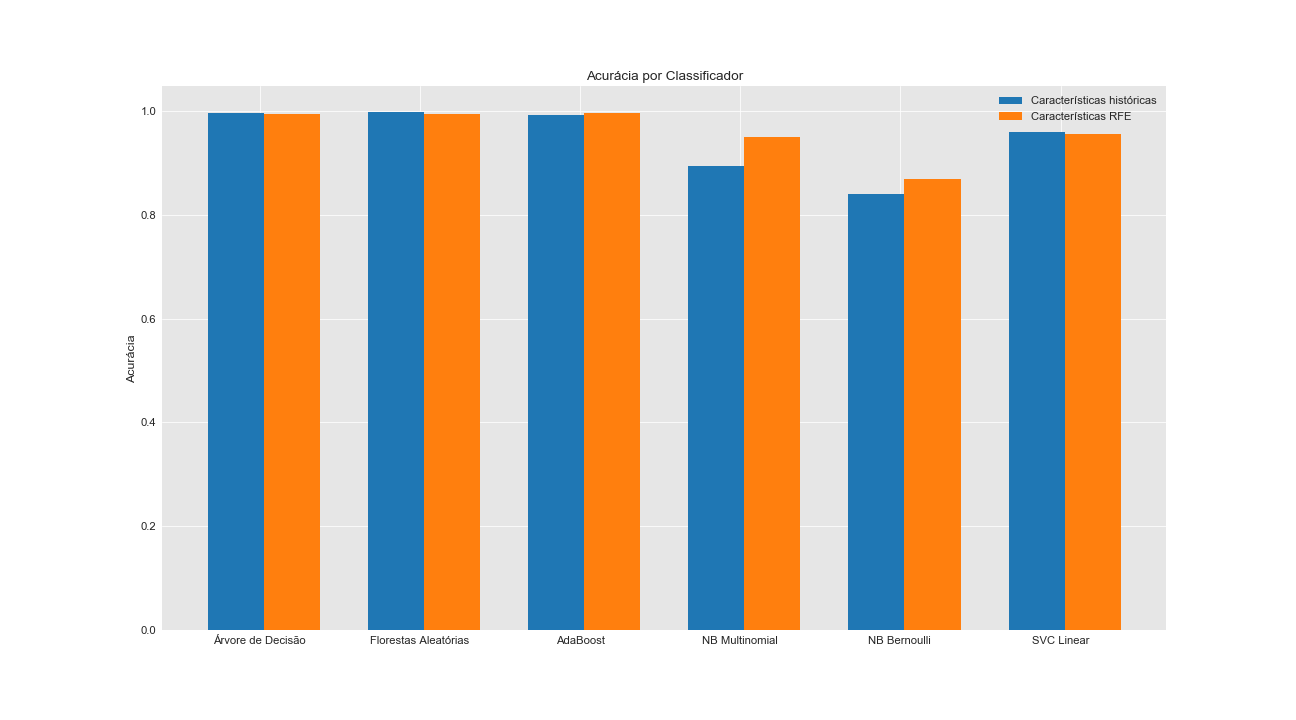
\includegraphics[scale=0.30]{figs/ComparativoAcuracias.png}
\label{r.graf1}
\legend{\small Fonte: Elaborada pelo autor.}
\end{figure}

\begin{figure}[h]
\caption{Comparativo de Número de Características.}
\centering
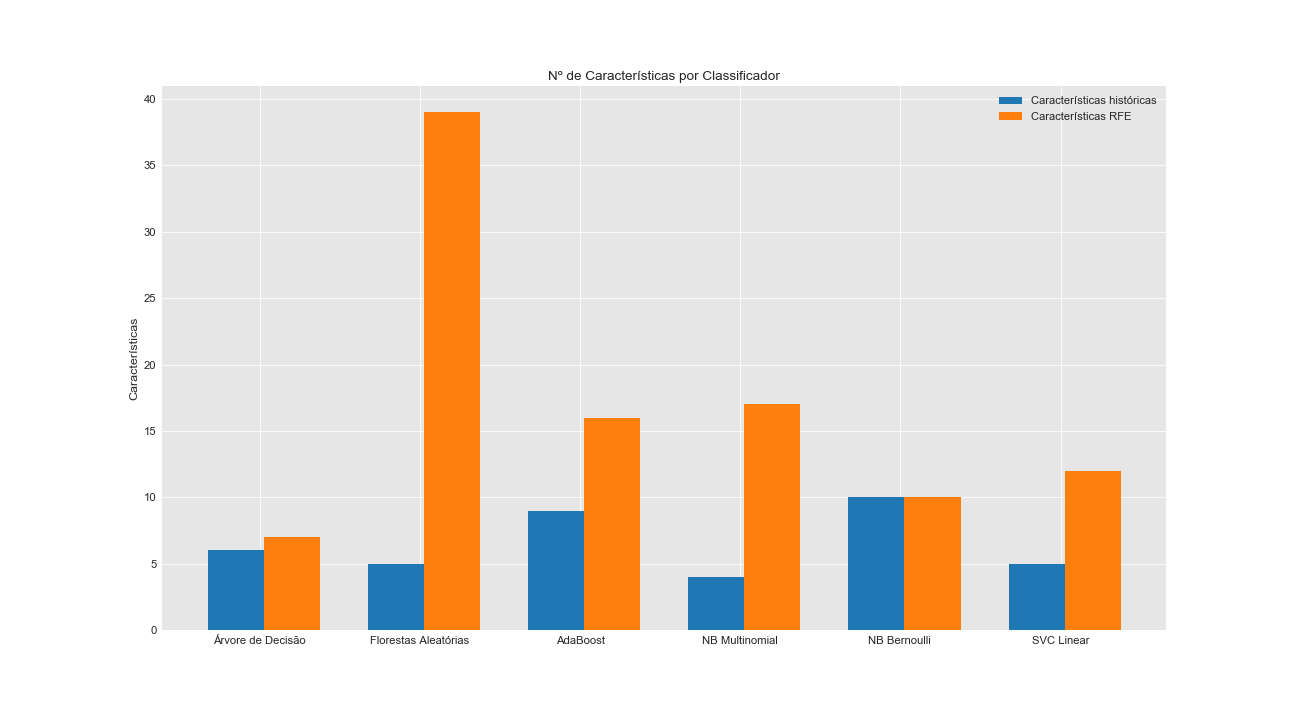
\includegraphics[scale=0.30]{figs/ComparativoCaracs.png}
\label{r.graf2}
\legend{\small Fonte: Elaborada pelo autor.}
\end{figure}

\section{Características}

Esta seção apresentará alguns gráficos que buscam ilustrar a distribuição de características presentes nas duas abordagens. A figura \ref{r.graf3} mostra a quantidade de vezes que uma característica foi utilizada pelos classificadores na abordagem de Força Bruta, enquanto as figuras \ref{r.graf4} e \ref{r.graf5} mostram as dez características que foram mais e menos utilizadas, respectivamente, na abordagem RFE. Por fim, o último gráfico mostra a frequência das características históricas na segunda abordagem de maneira isolada. 

\begin{figure}[h]
\caption{Frequência de Características na abordagem de Força Bruta.}
\centering
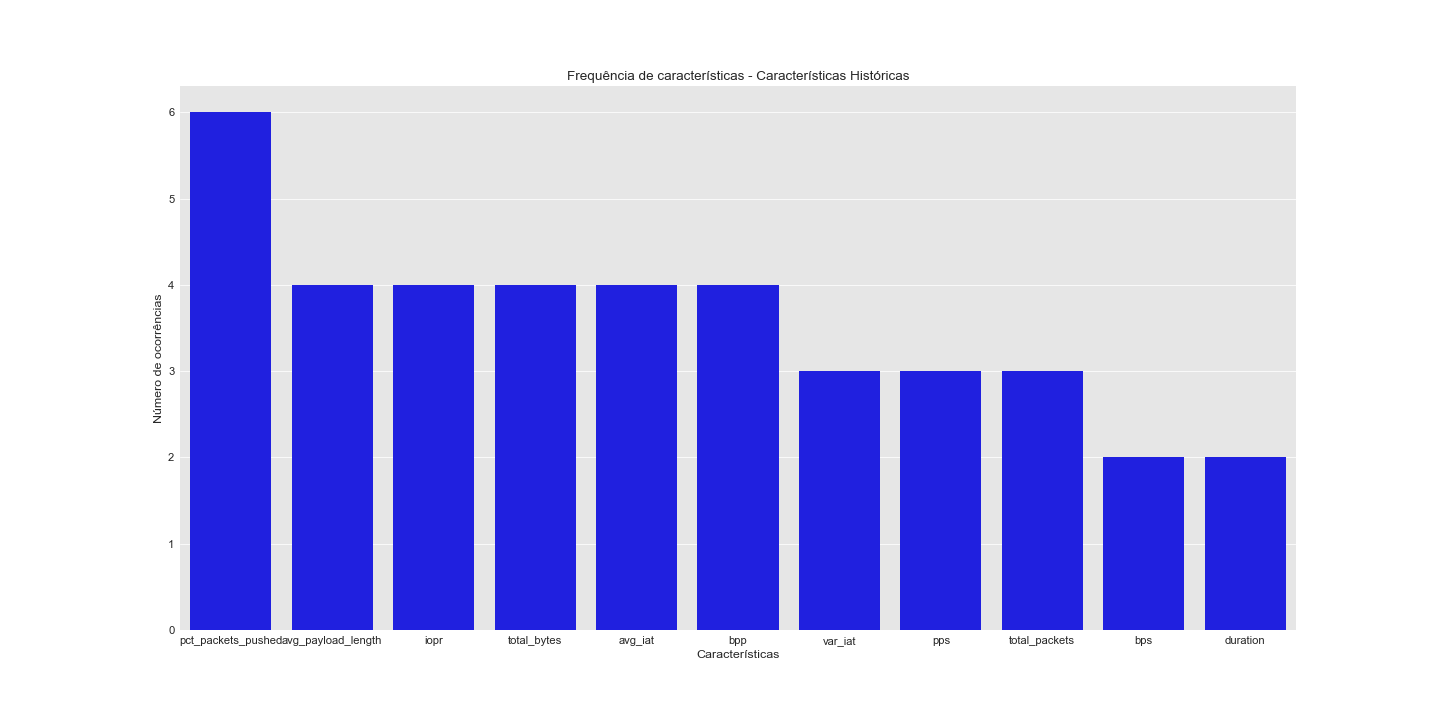
\includegraphics[scale=0.30]{figs/CaracteristicasMetodo1.png}
\label{r.graf3}
\legend{\small Fonte: Elaborada pelo autor.}
\end{figure}

\begin{figure}[h]
\caption{Características mais frequentes na abordagem de RFE.}
\centering
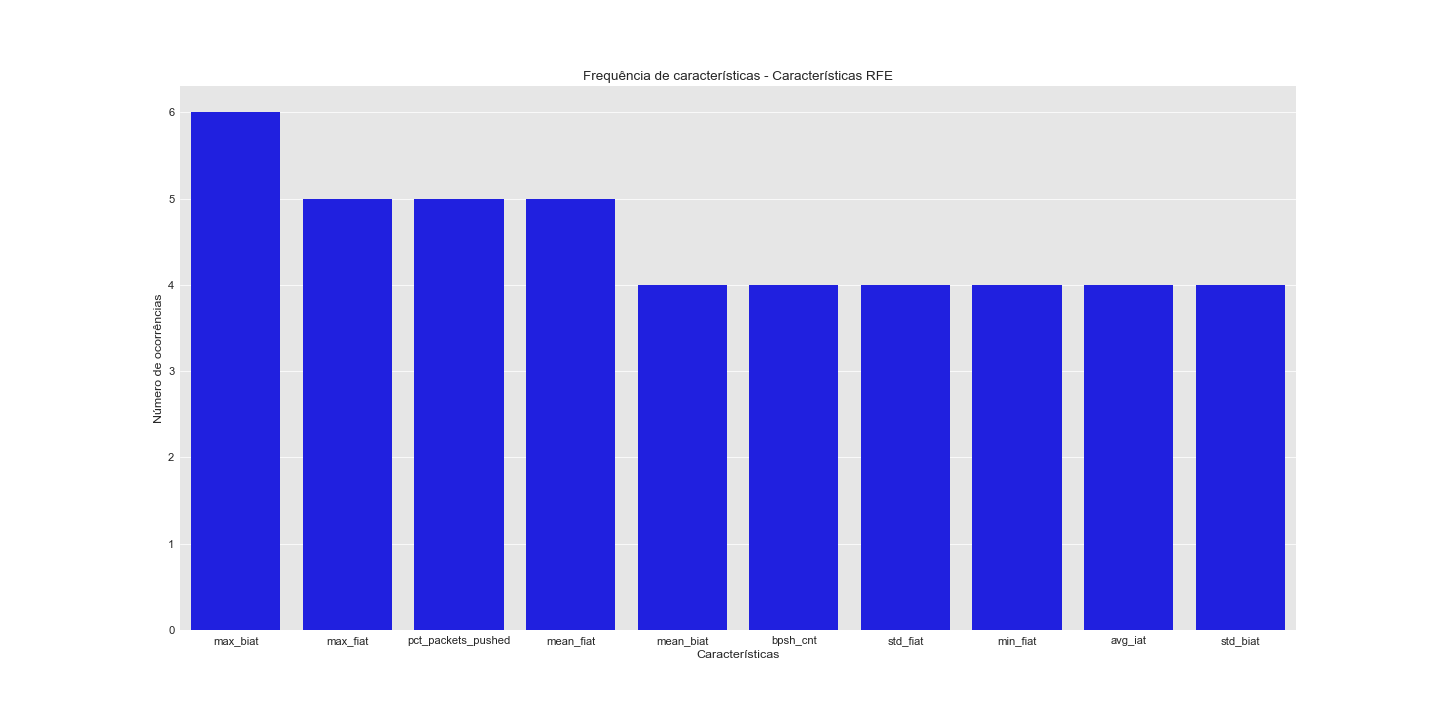
\includegraphics[scale=0.30]{figs/CaracteristicasMetodo2.png}
\label{r.graf4}
\legend{\small Fonte: Elaborada pelo autor.}
\end{figure}

\begin{figure}[h]
\caption{Características menos frequentes na abordagem de RFE.}
\centering
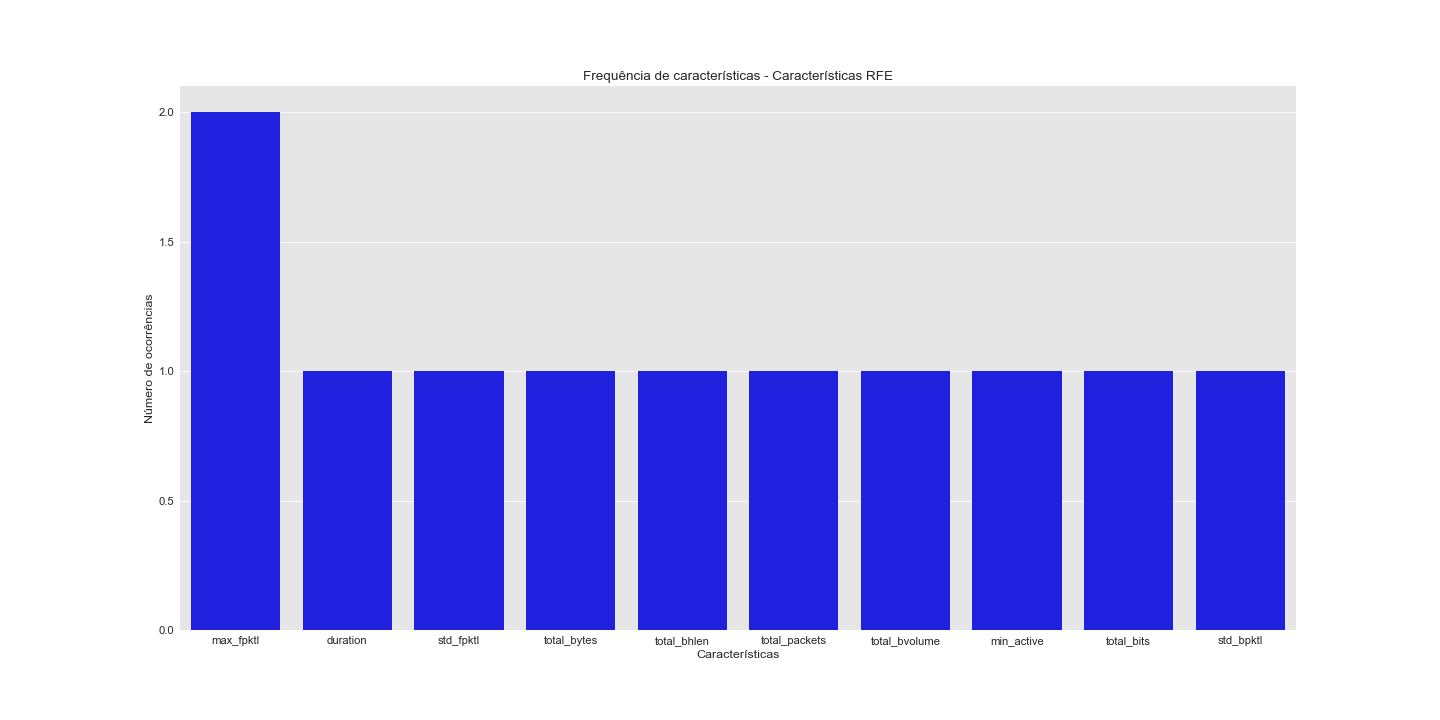
\includegraphics[scale=0.30]{figs/CaracteristicasMetodo2-menos.png}
\label{r.graf5}
\legend{\small Fonte: Elaborada pelo autor.}
\end{figure}

\begin{figure}[h]
\caption{Frequência de Características Históricas na abordagem de RFE.}
\centering
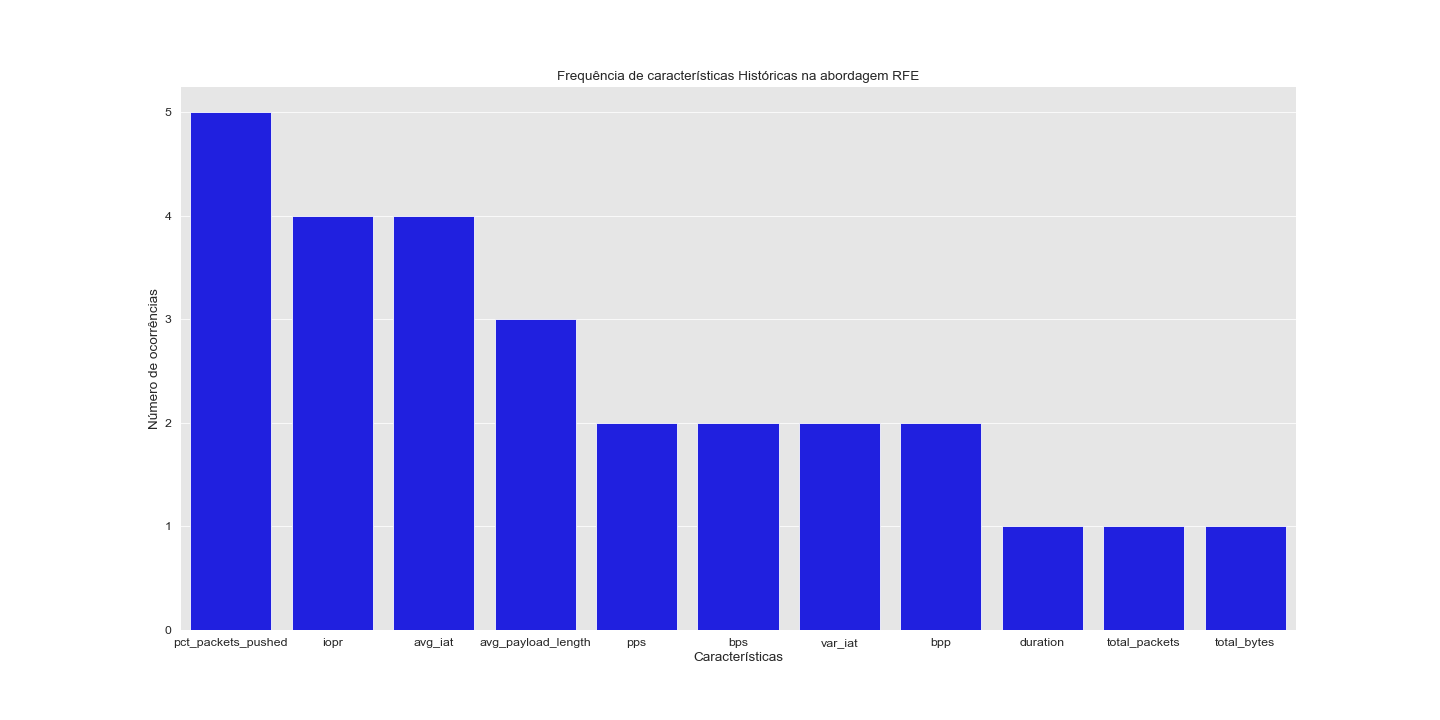
\includegraphics[scale=0.30]{figs/CaracteristicasSVM.png}
\label{r.graf6}
\legend{\small Fonte: Elaborada pelo autor.}
\end{figure}

\section{Hiper-parâmetros}

Esta seção irá apresentar os resultados obtidos pela otimização de Hiper-parâmetros feita para o algoritmo de SVM. A tabela \ref{r.t3} contém os valores de acurácia obtidos para cada Kernel, além dos parâmetros ótimos obtidos no processo. Por fim, a figura \ref{r.grafgrid} apresenta a variação na acurácia para cada Kernel.

\begin{table}[h!]
  \begin{center}
    \caption{Resultados da otimização de Hiper-parâmetros do SVM}
    \label{r.t3}
    \begin{tabular}{l|c|c} % <-- Alignments: 1st column left, 2nd middle and 3rd right, with vertical lines in between
      \textbf{Kernel} & \textbf{Acurácia} & \textbf{Parâmetros}\\
      \hline
      Linear & 0.996604 & C:100\\
      RBF & 0.978840 & C: 100,$\gamma$: 0.001\\
      Sigmoidal & 0.749477 & C: 10,$\gamma$: 0.0001, r:0\\
    \end{tabular}
  \end{center}
\end{table}

\begin{figure}[h]
\caption{Comparativo de Acurácia dos Kernels do SVM.}
\centering
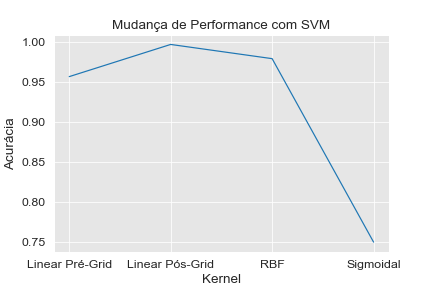
\includegraphics[scale=0.7]{figs/Hiperparametros.png}
\label{r.grafgrid}
\legend{\small Fonte: Elaborada pelo autor.}
\end{figure}
\chapter{Conclusão}
\label{c.conclusao}

Esta monografia fez uma análise sobre a utilização de técnicas da área de \textit{Machine Learning} para a detecção de \textit{Botnets} baseadas no protocolo IRC em uma rede, através da análise fluxos bidirecionais. Estudos deste tipo se fazem cada vez mais relevante tendo em vista o crescimento do uso de aparelhos conectados em rede que podem ser integrados às \textit{botnets}, aumentando ainda mais o poder de seus ataques.

Sendo assim, é possível afirmar que o presente estudo cumpriu seus objetivos ao estudar a aplicação e eficiência de vários algoritmos da área, além de explorar a utilização de características utilizadas em estudos passados e ainda explorar novas possibilidades de uso. 

Com base nos resultados, é possível afirmar que os classificadores testados foram bem sucedidos em suas tarefas, obtendo altos níveis de acurácia. Dentre eles destacam-se os métodos baseados em Árvores, que obtiveram os melhores resultados, seguidos pelos métodos de \textit{Support Vector Machines}, e por último pelos métodos de \textit{Naive Bayes}.

Com relação às duas abordagens de utilização de características, é possível observar que a utilização do RFE para seleção de características impactou diretamente na melhoria da acurácia dos modelos probabilísticos de Naive Bayes, no entanto para os outros métodos os resultados foram parecidos. Porém, a utilização do RFE ainda apresenta menor custo computacional, o que a torna mais efetiva.

Já para o número de características, percebe-se que nenhum deles apresentou uma diferença muito grande com exceção do método de Florestas Aleatórias que acabou utilizando todas as características presentes no conjunto, e assim utilizando 34 características a mais que na abordagem de Força Bruta. Para a primeira abordagem, utilizando 11 características foi obtida uma média de 6,5 características utilizadas por classificador, enquanto para a segunda utilizando 39 características observou-se uma média de 16,8 características.

As características que foram utilizadas nos estudos anteriores se fizeram muito presente nas encontradas pelo RFE, com destaque para algumas que se destacaram em ambas as abordagem: Porcentagem de Pacotes Enviados, IOPR, Média de tamanho do Payload, e o tempo de chegada entre pacotes médio, ou IAT médio. 

Observa-se ainda que no que tange a abordagem do RFE, de maneira geral características ligadas a IAT foram amplamente usadas por quase todos os classificadores, enquanto as características de tamanho de fluxo, como total de bytes, não obtiveram muita representatividade em ambas as abordagens, assim como a característica duração do fluxo.

Por fim, foi possível observar o impacto que a otimização de hiper-parâmetros pode ter no desempenho do SVM, tendo em vista que a troca do valor de seu parâmetro C levou a um considerável aumento em sua acurácia. Além disso, também demonstrou que o Sigmoidal se saiu significativamente pior do que o Linear e o RBF para este tipo de problema.

\section{Trabalhos Futuros}

Como trabalhos futuros baseados neste estudo, têm-se a exploração de outras características possíveis de serem utilizadas na área, avaliar a eficiência dos métodos e características descritos para outros protocolos de \textit{Botnet} centralizadas como o HTTP que vem crescendo em uso recentemente ou descentralizadas que utilizam comunicação P2P, implementação de outras técnicas da área, como Redes Neurais Artificiais ou algoritmos de  ML não-supervisionado para encontrar padrões na rede, trabalhar com outras bases de dados, que apresentem maior volume de pacotes, e implementação de um sistema de monitoramento que analise os fluxos em tempo real.
% --------------------------------------------------------
% ELEMENTOS PÓS-TEXTUAIS
% --------------------------------------------------------

\postextual


% --------------------------------------------------------
% REFERÊNCIAS BIBLIOGRÁFICAS
% --------------------------------------------------------

\bibliography{referencias}


% --------------------------------------------------------
% GLOSSÁRIO
% --------------------------------------------------------

% Consulte o manual da classe abntex2 para orientações sobre o glossário.
%\glossary


% --------------------------------------------------------
% APÊNDICES
% --------------------------------------------------------

% Inicia os apêndices
%\begin{apendicesenv}
% Imprime uma página indicando o início dos apêndices
%\partapendices
% Criação do apêndice
%\end{apendicesenv}


% --------------------------------------------------------
% ÍNDICE REMISSIVO
% --------------------------------------------------------

\printindex


% --------------------------------------------------------
% FINAL DO DOCUMENTO
% --------------------------------------------------------

\end{document}
